
\chapter{Conception et implémentation de l'application}
\section{Introduction}
Après avoir étudié les différents techniques utilisés pour le développement des applications mobiles, on va entamer dans ce chapitre la partie conception et implémentation de notre application Android en fixant les objectifs de cette application suivie par une étude comparative sur des solutions déjà existantes, ensuite on va présenter les diagrammes UML ainsi que le diagramme d'action, puis les maquettes fonctionnelles et les interfaces utilisateur. À la fin on termine avec les outils matériels et logiciels utilisés au long du cursus du développement de l’application.
\section{Conception}
\subsection{Objectif du projet}
Ce projet a pour but de développer une application mobile sous la plateforme Android. qui permettra d'afficher dans une carte géographique des restaurants qui sont à proximité de l'utilisateur avec les informations de ces derniers ainsi que les menus qui lui seront accessible tous ça a pour but de rendre la recherche sur les restaurants et les menus plus facile et efficace .
\subsection{Applications déja existantes}
\paragraph*{}
Il existe peu d'applications mobiles dans le domaine de la restauration nous allons explorer certaines des plus populaires solutions existantes aujourd’hui.

\newpage
\subsubsection{TripAdvisor}
\begin{wrapfigure}[8]{r}{2cm}
    \vspace{-15pt}
    
\includegraphics[width=2cm]{images/Chapitre1/tripadvisor.png}
    \vspace{-20pt}
    \caption{{\footnotesize Logo de TripAdvisor}}
\end{wrapfigure}

TripAdvisor est une plate-forme disponible en web et en application mobile, cette plate-forme offre des avis et des suggestions d'hôtels, lieux de loisirs, villes et régions à l'échelle internationale, compare les prix et affiche les meilleures offres du moment.

TripAdvisor couvre aussi les services de restauration et fournit des informations sur les différents restaurants qui existent dans le monde entier. \bigskip

Le service qu'offre cette plate-forme pour le secteur de la restauration a des avantages : \bigskip

	\tab- L'utilisation de ce service est gratuite.\medskip

	\tab- Donne un aperçu sur les restaurants et offre des informations sur la fourchette des prix..\medskip

	\tab- Des évaluations et des avis sont fournis par les utilisateurs eux-mêmes.\bigskip

TripAdvisor a ses avantages mais aussi ses inconvénients:\bigskip

	\tab- On ne peut pas parcourir les restaurants en utilisant une carte géographique.\medskip

	\tab- L'utilisation d'une application tierce est indispensable pour avoir l'itinéraire vers les restaurants.\medskip

	\tab- Les informations offertes par cette plate-forme sont limitées au avis fourni par les utilisateurs.
 

	\begin{figure}[!ht]

		\centering
		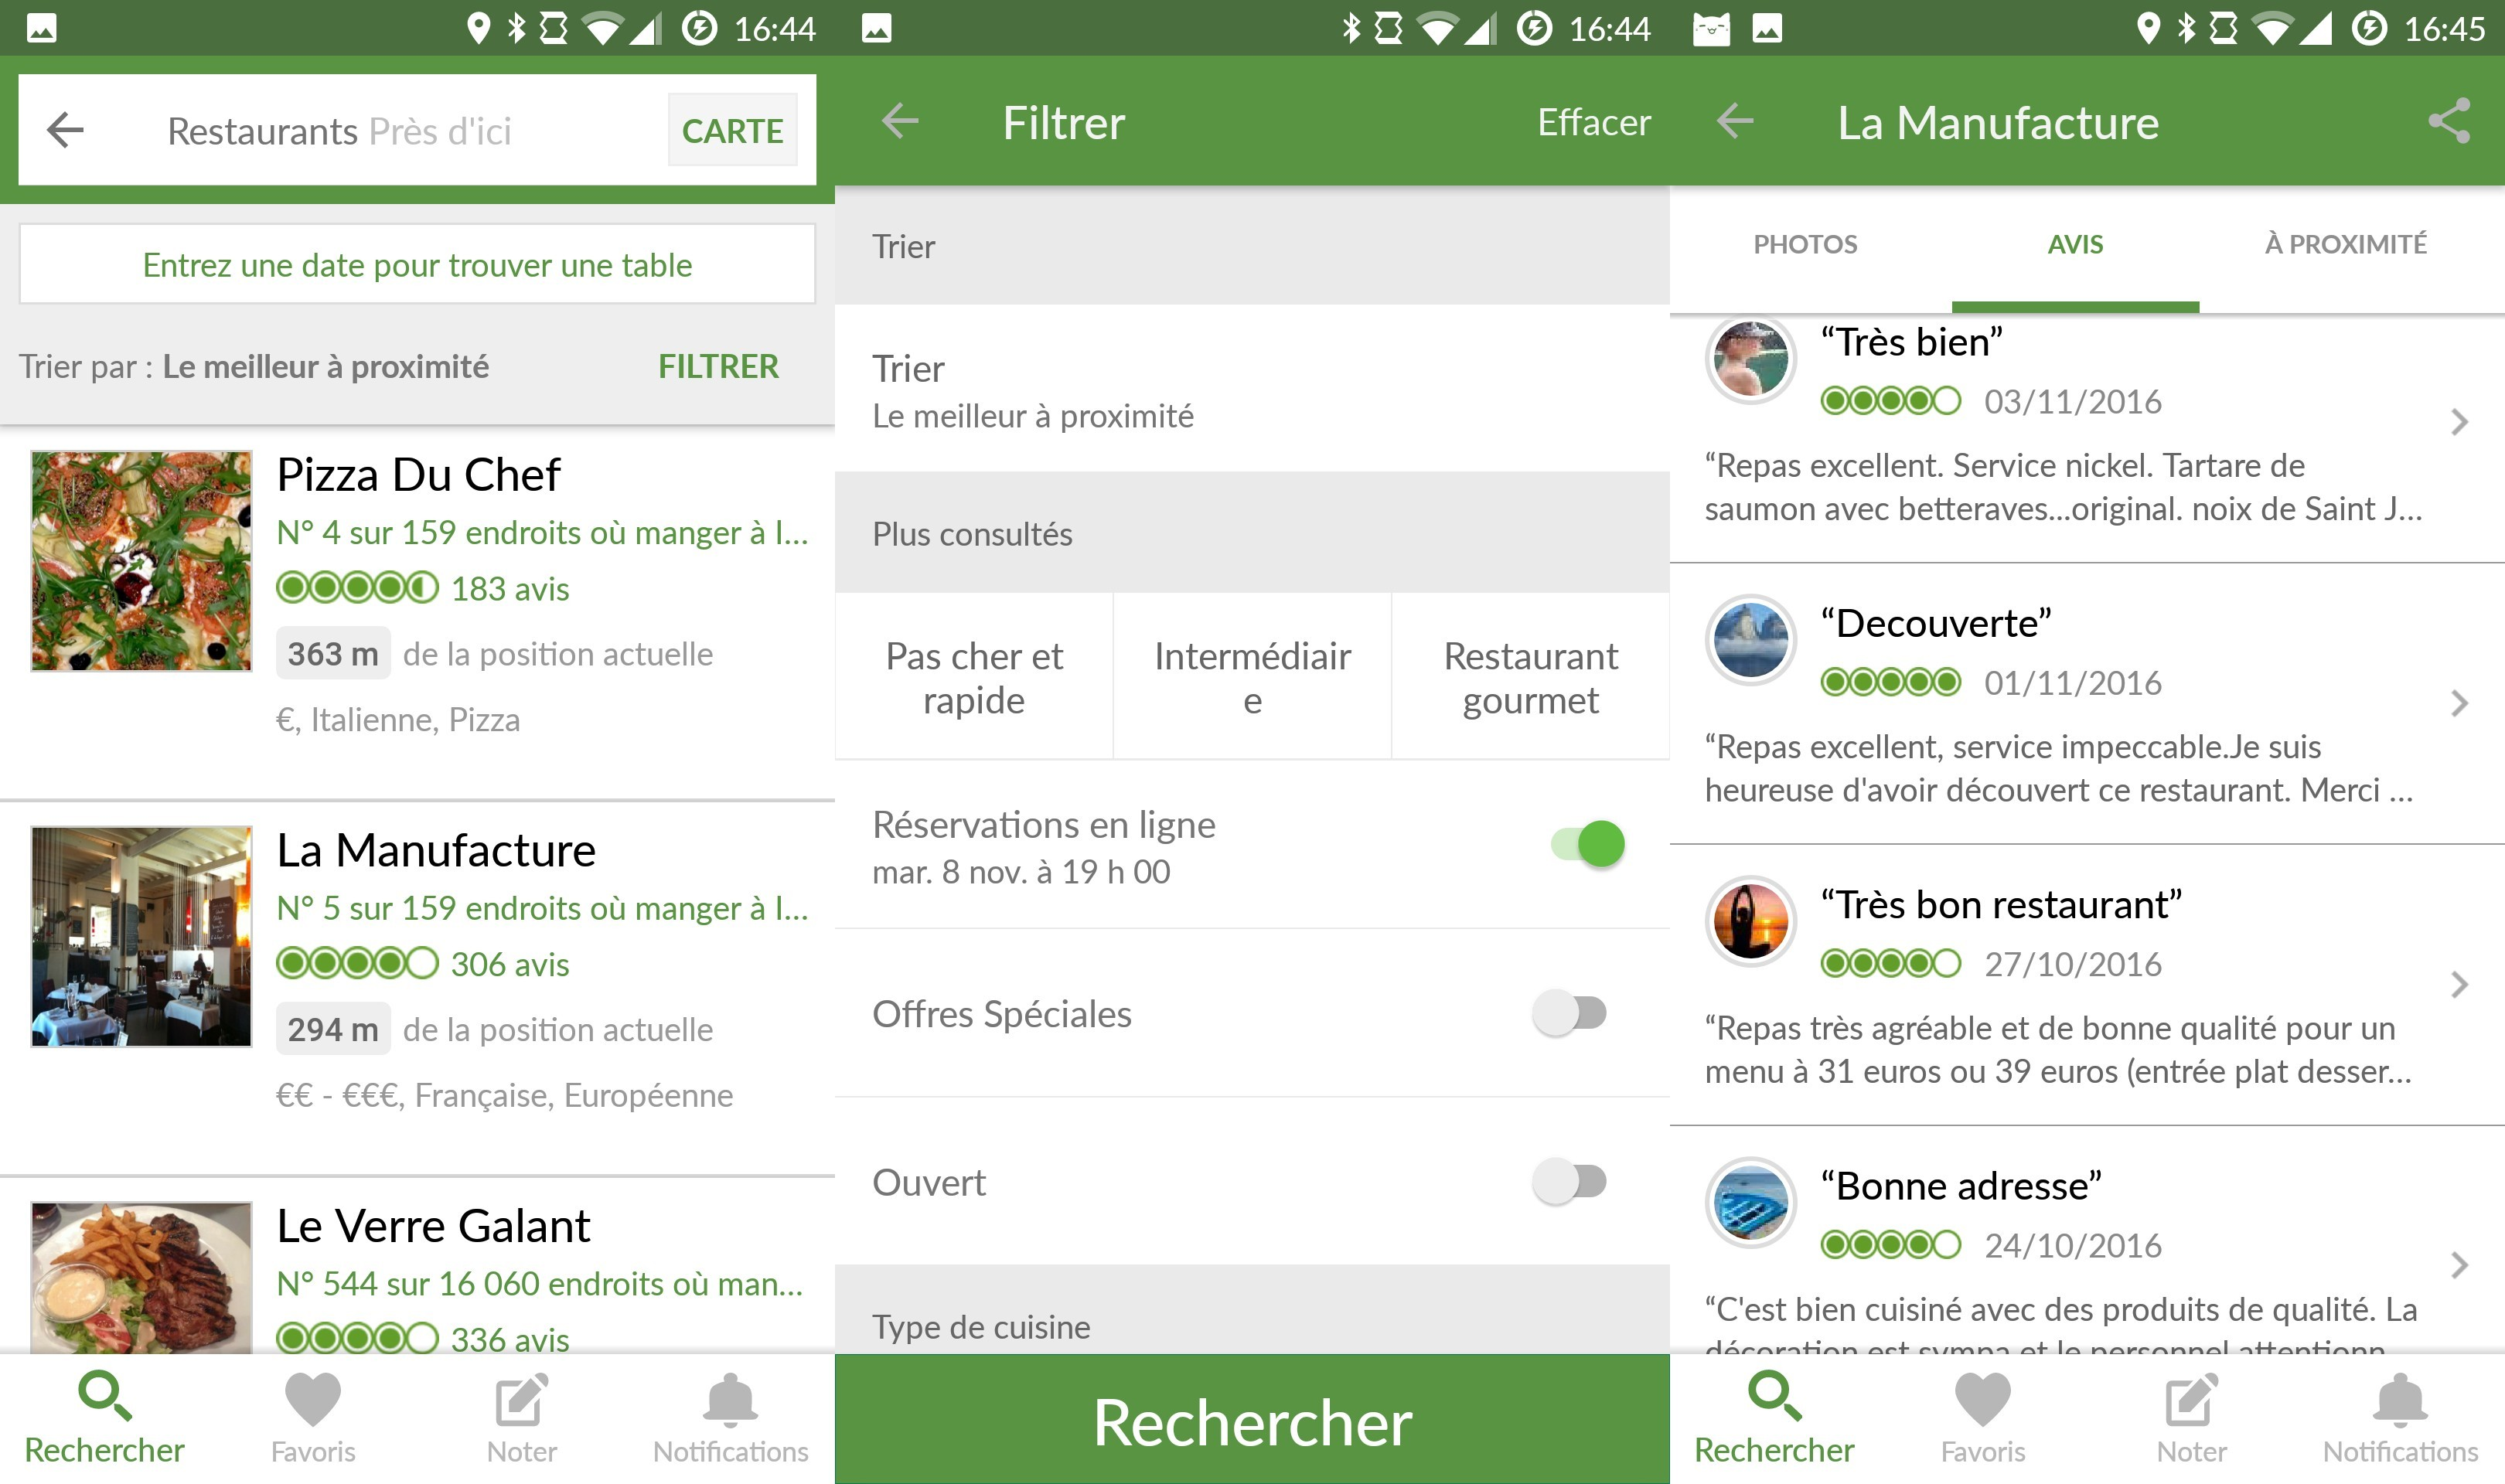
\includegraphics[width=4in]{images/Chapitre1/trip_advisor.jpeg}
		\label{fig:tripadvisor}
		\caption{Interface de TripAdvisor lors de la recherche des restaurants et les avis}
	 \end{figure}
\newpage
\subsubsection{Google Maps}
\begin{wrapfigure}[8]{r}{2cm}
	\vspace{-15pt}
	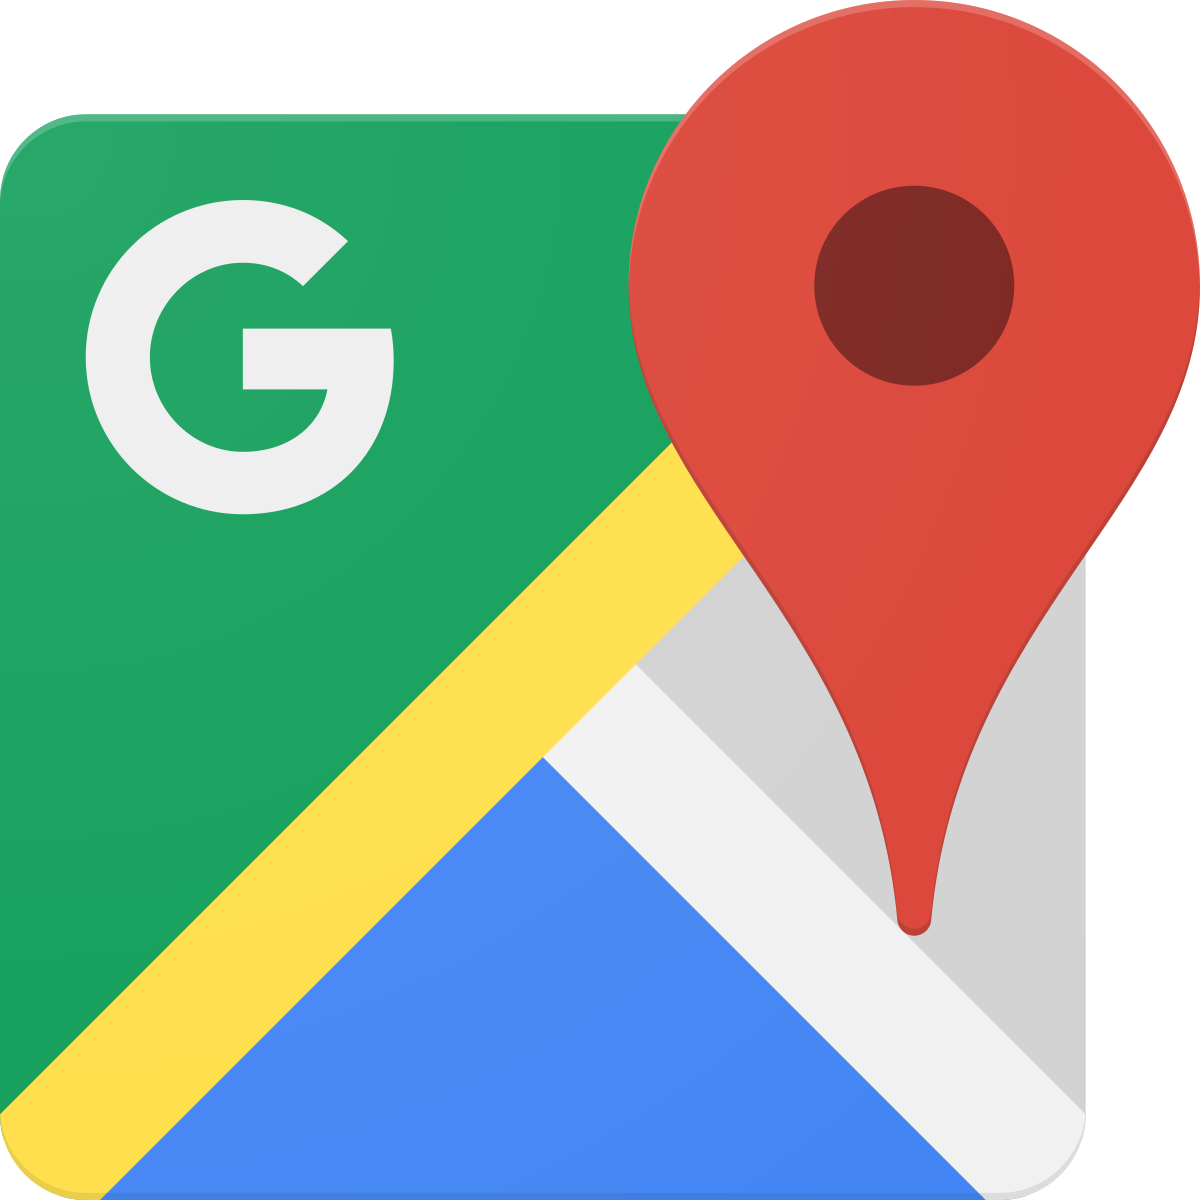
\includegraphics[width=2cm]{images/Chapitre1/googlemaps.png}
	\vspace{-20pt}
	\caption{{\footnotesize Logo de Google Maps}}
 \end{wrapfigure}
Google maps est un service de cartographie développé par l'entreprise Google et lancé en 2005. Ce service offre différents types de vues et permet aussi d'afficher les différents points d'intérêts dans le monde comme les hôtels, les lieux d'attractions, etc. Ce qui nous intéresse dans notre domaine de recherche est la géolocalisation des restaurants, une fonctionnalité qu'offre ce service.

En accédant au site web ou l'application mobile, l'utilisateur aura accès à un large choix de restaurants proposés grâce à un système de suggestions, aussi développé par Google. L'utilisateur pourra donc accéder aux informations des restaurants ainsi que des photos et des avis généralement postés par la communauté des utilisateurs de Google Maps.
\subparagraph*{}
Google Maps présente de nombreux avantages, nous en citerons :\bigskip
 
	\tab- L'utilisation de ce service est gratuite.\medskip

	\tab- La plupart des restaurants sont affichés dans la carte.\medskip

	\tab- Les images des restaurants sont parfois affichées.\medskip
	
	\tab- Les utilisateurs peuvent donner des avis et des notes.\medskip

	\tab- Des itineraires precis sont proposés.\bigskip

	
Néanmoins ce service présente aussi des inconvénients:\bigskip

	\tab- Les menus detaillés ne sont pas affichés dans l'interface.\medskip

	\tab- On ne peut pas filtrer les types de restaurants.\medskip


	\begin{figure}[!ht]

		\centering
		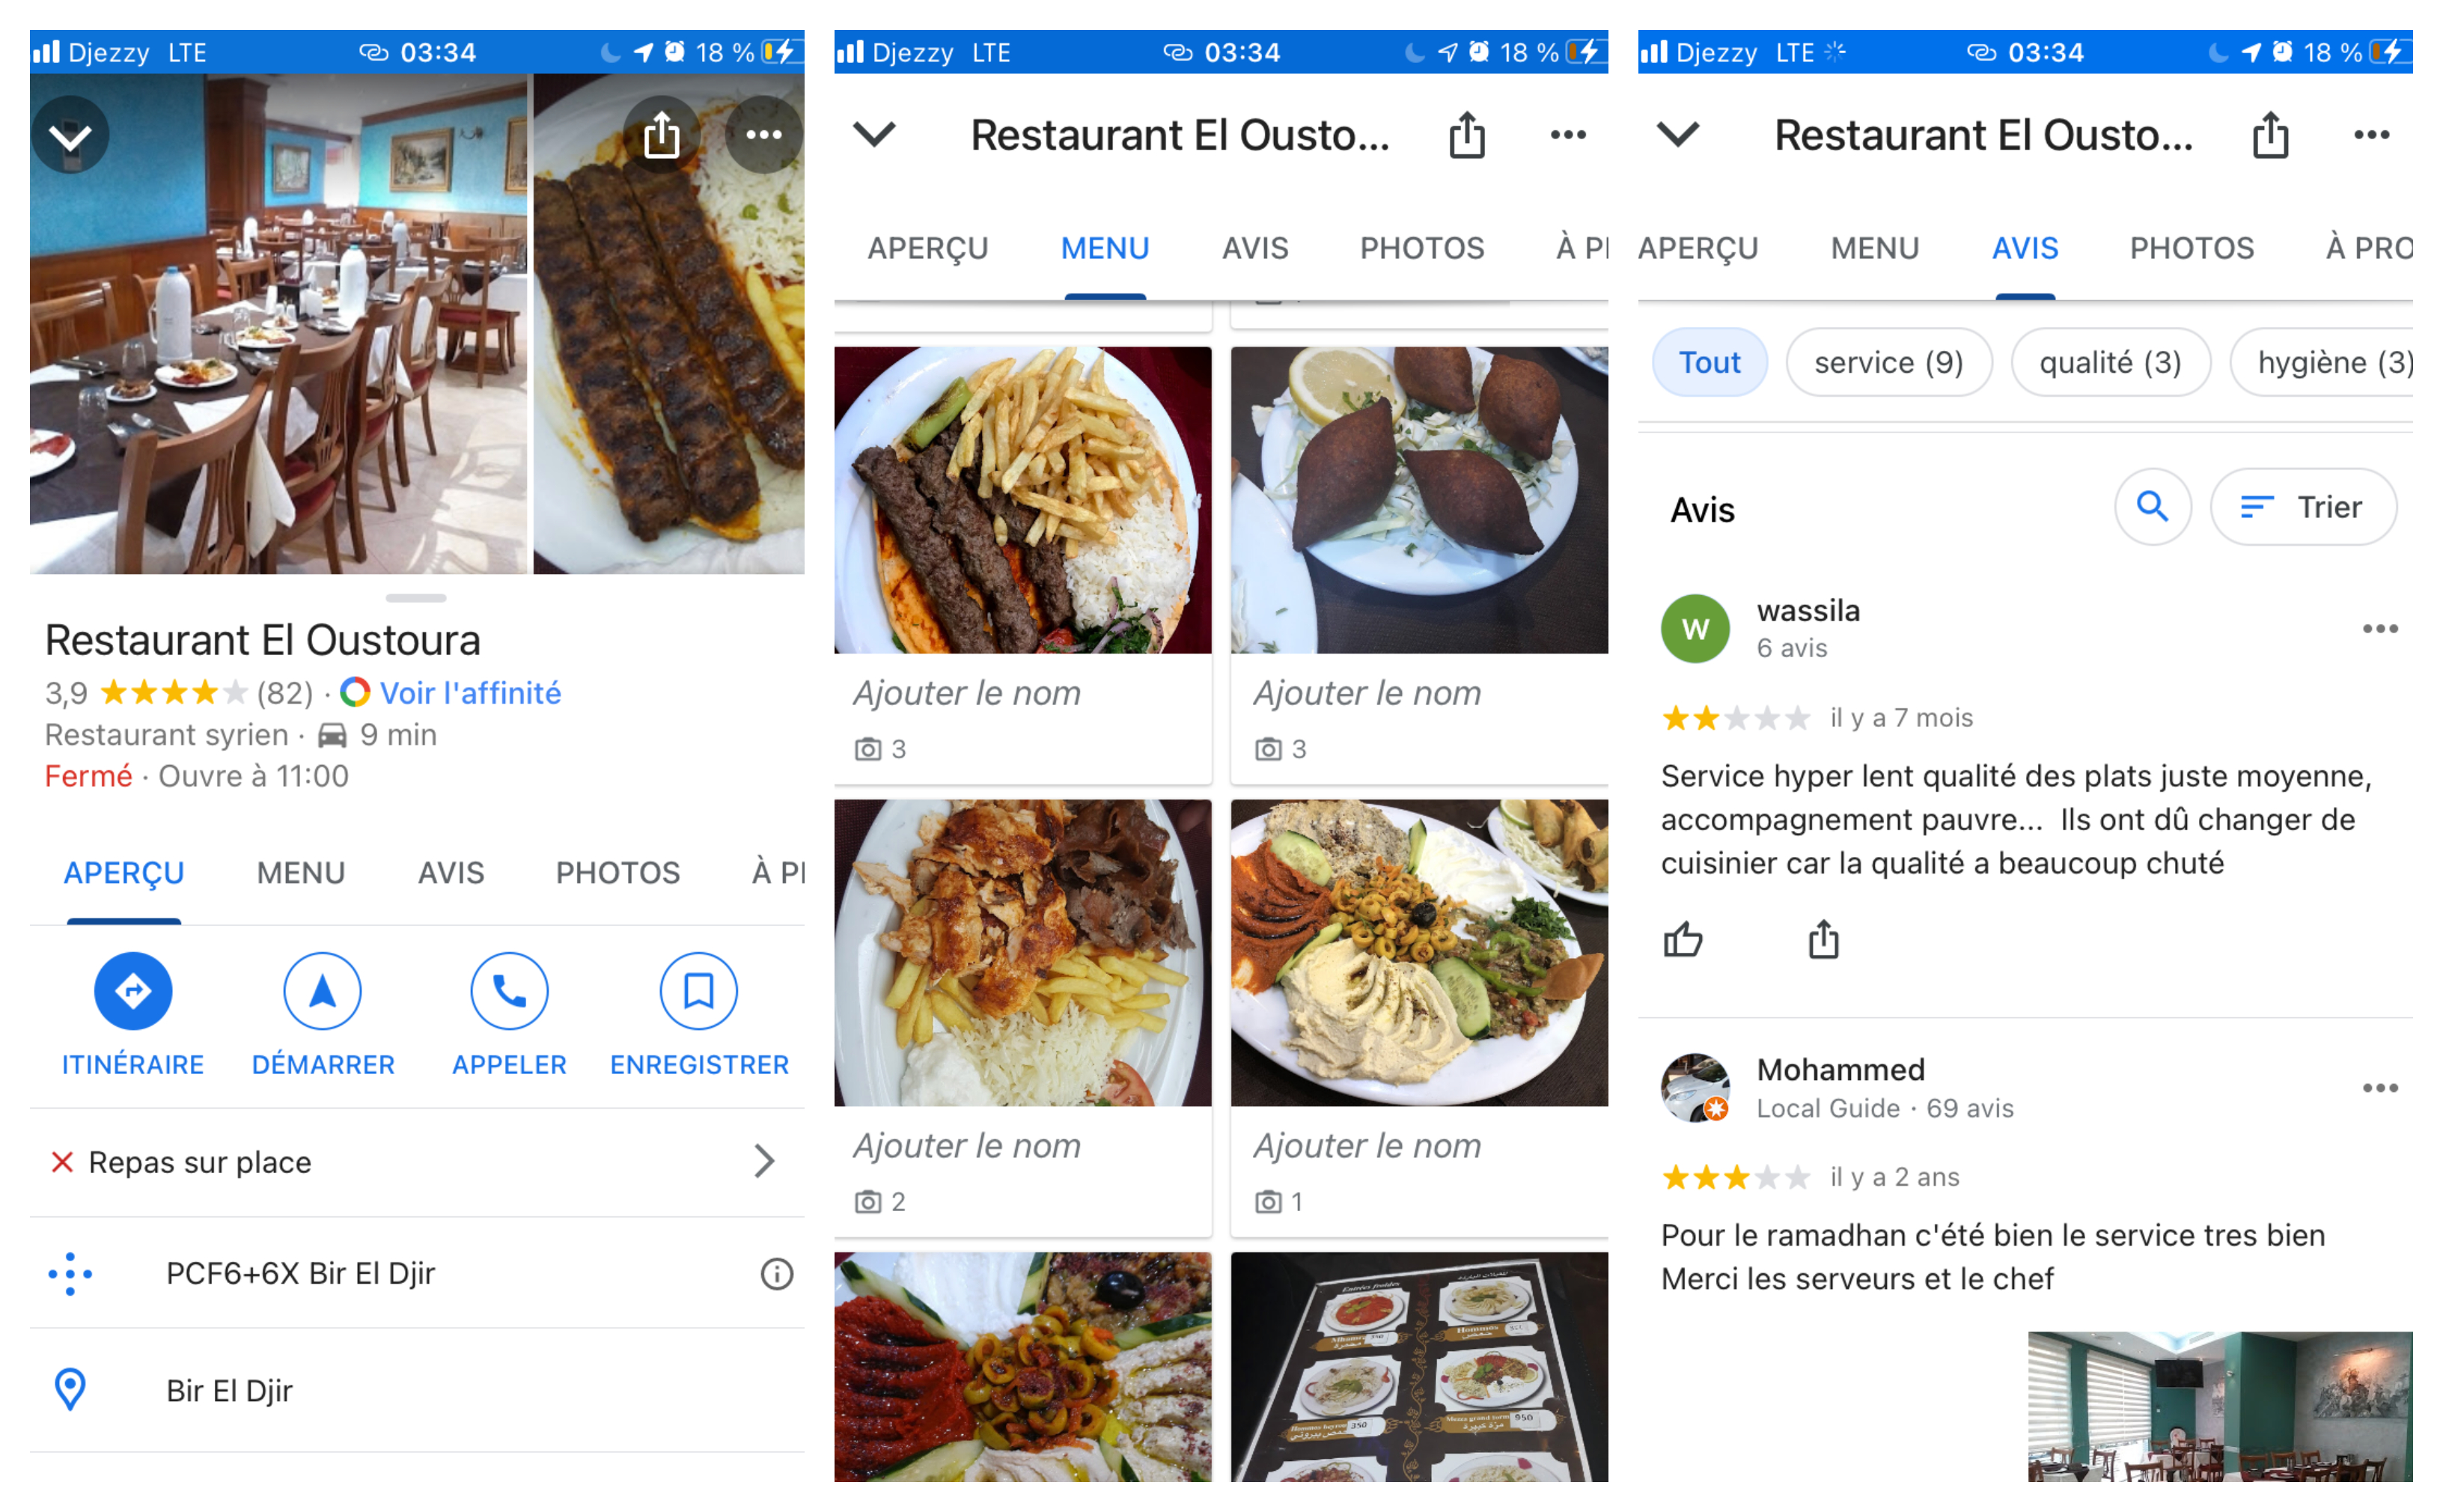
\includegraphics[width=4.5in]{images/Chapitre1/page_resto.jpg}
		\label{fig:pageresto}
		\caption{Exemple de différents ecrans lors d'une recherche d'un restaurant }
	 \end{figure}
	 
\newpage

\subsubsection{LaFourchette}
TheFork de son ancien nom "LaFourchette" est une plate-forme française de réservation de restaurants en ligne, accessible par un site web et par une application mobile disponible sur Android et iOS. Elle est présente dans plus de vingt pays en Europe et en Amérique latine.~\cite{TheFork2020}
\subparagraph*{}
\begin{wrapfigure}[8]{r}{3cm}
    \vspace{-15pt}
    
\includegraphics[width=3cm]{images/Chapitre1/lafourchette.jpg}
    \vspace{-20pt}
    \caption{{\footnotesize Logo de LaFourchette}}
\end{wrapfigure}

\subparagraph*{}
TheFork a ces avantages et ces inconvénients, parmi ces avantages on a :\bigskip

	\tab- La base de données regroupe plus de 80000 restaurants a travers le monde.~\cite{RestaurantsSiteReservation} \medskip

	\tab- L'application est multiplate-forme et disponible en version web et mobile. \medskip

	\tab- L'interface utilisateur est simple qui permet d'utiliser le service de manière efficace. \medskip

	\tab- La présence de la fonction d'exploration des restaurants via une carte.\bigskip

Quant aux Inconvénients nous citeront :\bigskip

	\tab- Le service n'est pas totalement gratuit.\medskip

	\tab- Cette application est dédiée qu'aux réservations de restaurans et ne donne pas des informations détaillées sur les menus.\medskip

	\tab- L'application ne prends pas encore en charge les restaurans algeriens. \medskip

   



\subsection{Les diagrammes UML}
Le langage UML est un langage de modélisation visuelle commun,
et riche sémantiquement et syntaxiquement. Il est destiné à 
l'architecture, la conception et la mise en œuvre de systèmes logiciels complexes par leur structure aussi bien que leur comportement.
Il ressemble aux plans utilisés dans d'autres domaines et se 
compose de différents types de diagrammes. Dans l'ensemble, 
les diagrammes UML décrivent la limite, la structure et le 
comportement du système et des objets qui s'y trouvent.

L'UML n'est pas un langage de programmation, mais il existe des outils qui peuvent être utilisés pour générer du code en plusieurs langages à partir de diagrammes UML. L'UML a une relation directe avec l'analyse et la conception orientées objet.\\
Pour bien expliquer le fonctionnement de notre application et modéliser les diagrammes. On a utilisé l'outil Visual Paradigm Online qui est facile à manipuler afin de réaliser ces diagrammmes.
\newpage
\subsubsection{Diagrammes de séquence}
Enchainement des actions pour le lancement de l'application
\begin{figure}[!ht]

    \centering
    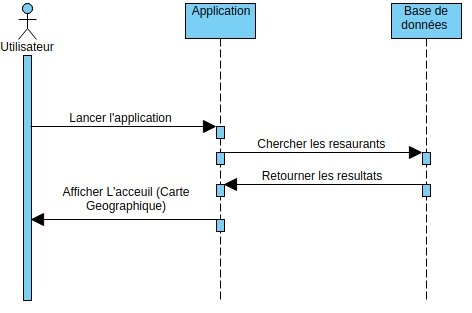
\includegraphics[width=5in]{images/Chapitre3/enchainement_lancement_application.jpg}
    \label{fig:umllancement}
    \caption{Enchainement des actions pour le lancement de l'application}
\end{figure}

\begin{figure}[!ht]

    \centering
    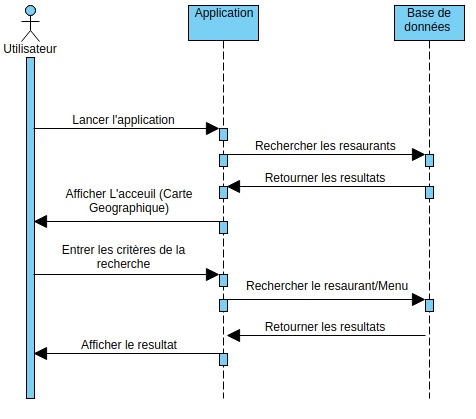
\includegraphics[width=4in]{images/Chapitre3/enchainement_recherche_resto_menu.jpg}
    \label{fig:label1}
    \caption{Enchainement des actions pour la recherche des restaurants}
\end{figure}

\begin{figure}[!ht]

    \centering
    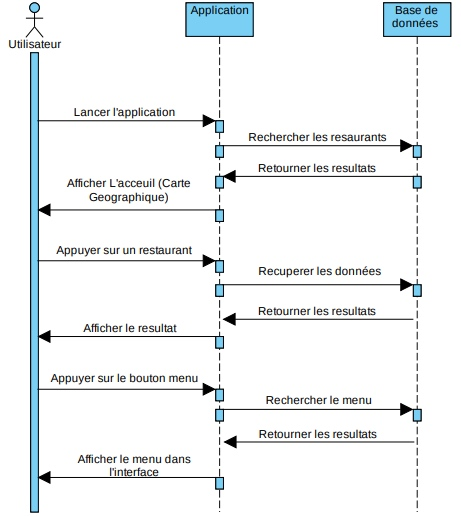
\includegraphics[width=3in]{images/Chapitre3/enchainement_affichage_resto_menu.jpg}
    \label{fig:label2}
    \caption{Enchainement des actions pour l'affichage de la page restaurant et son menu}
\end{figure}

\newpage
\subsubsection{Diagramme d'action}
\begin{figure}[!ht]

    \centering
    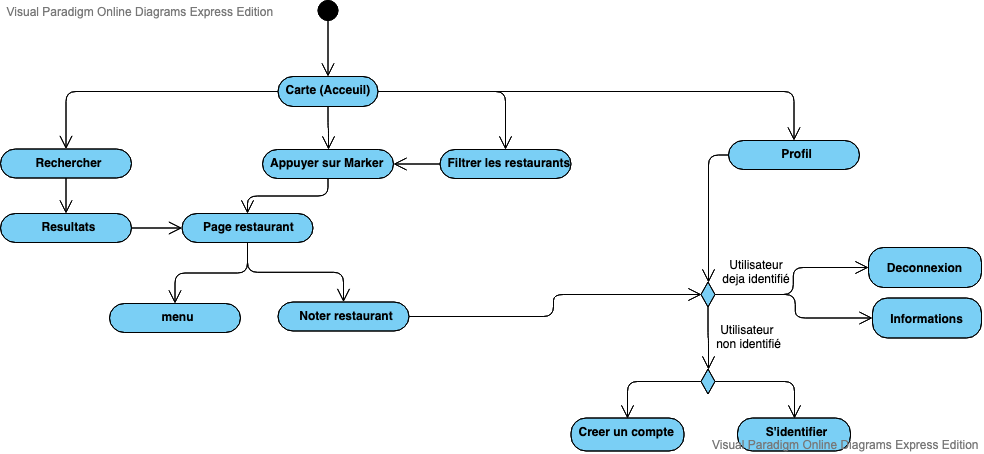
\includegraphics[width=6in]{images/Chapitre3/Diagramme_action.png}
    \label{fig:label3}
    \caption{Diagramme d'actions}
\end{figure}


\newpage
\subsection{Maquette fonctionelle (Wireframe)}
\subsubsection{Définition} La maquette fonctionelle ou Wireframe est
un schéma utilisé lors de la conception des interfaces des applications
pour définir les emplacements des  zones de texte, des images, des vidéos, des liens,
ainsi que des différents éléments graphiques.
\subsubsection{Outil utilisé}
Balsamiq Wireframes est une application de création d'interface 
utilisateur graphique ,elle permet au concepteur d'organiser des 
widgets prédéfinis à l' aide d'un éditeur WYSIWYG par glisser-
déposer .L'application est proposée dans une version de bureau 
ainsi qu'un plug-in pour Google Drive ~\cite{Balsamiq2020}.
\begin{figure}[!h]

    \centering
    
\includegraphics[width=4cm]{images/Chapitre3/balmockups.png}
    \label{fig:logobalsamiq}
    \caption{Logo de Balsamiq}
\end{figure}
\begin{figure}[!h]

    \centering
    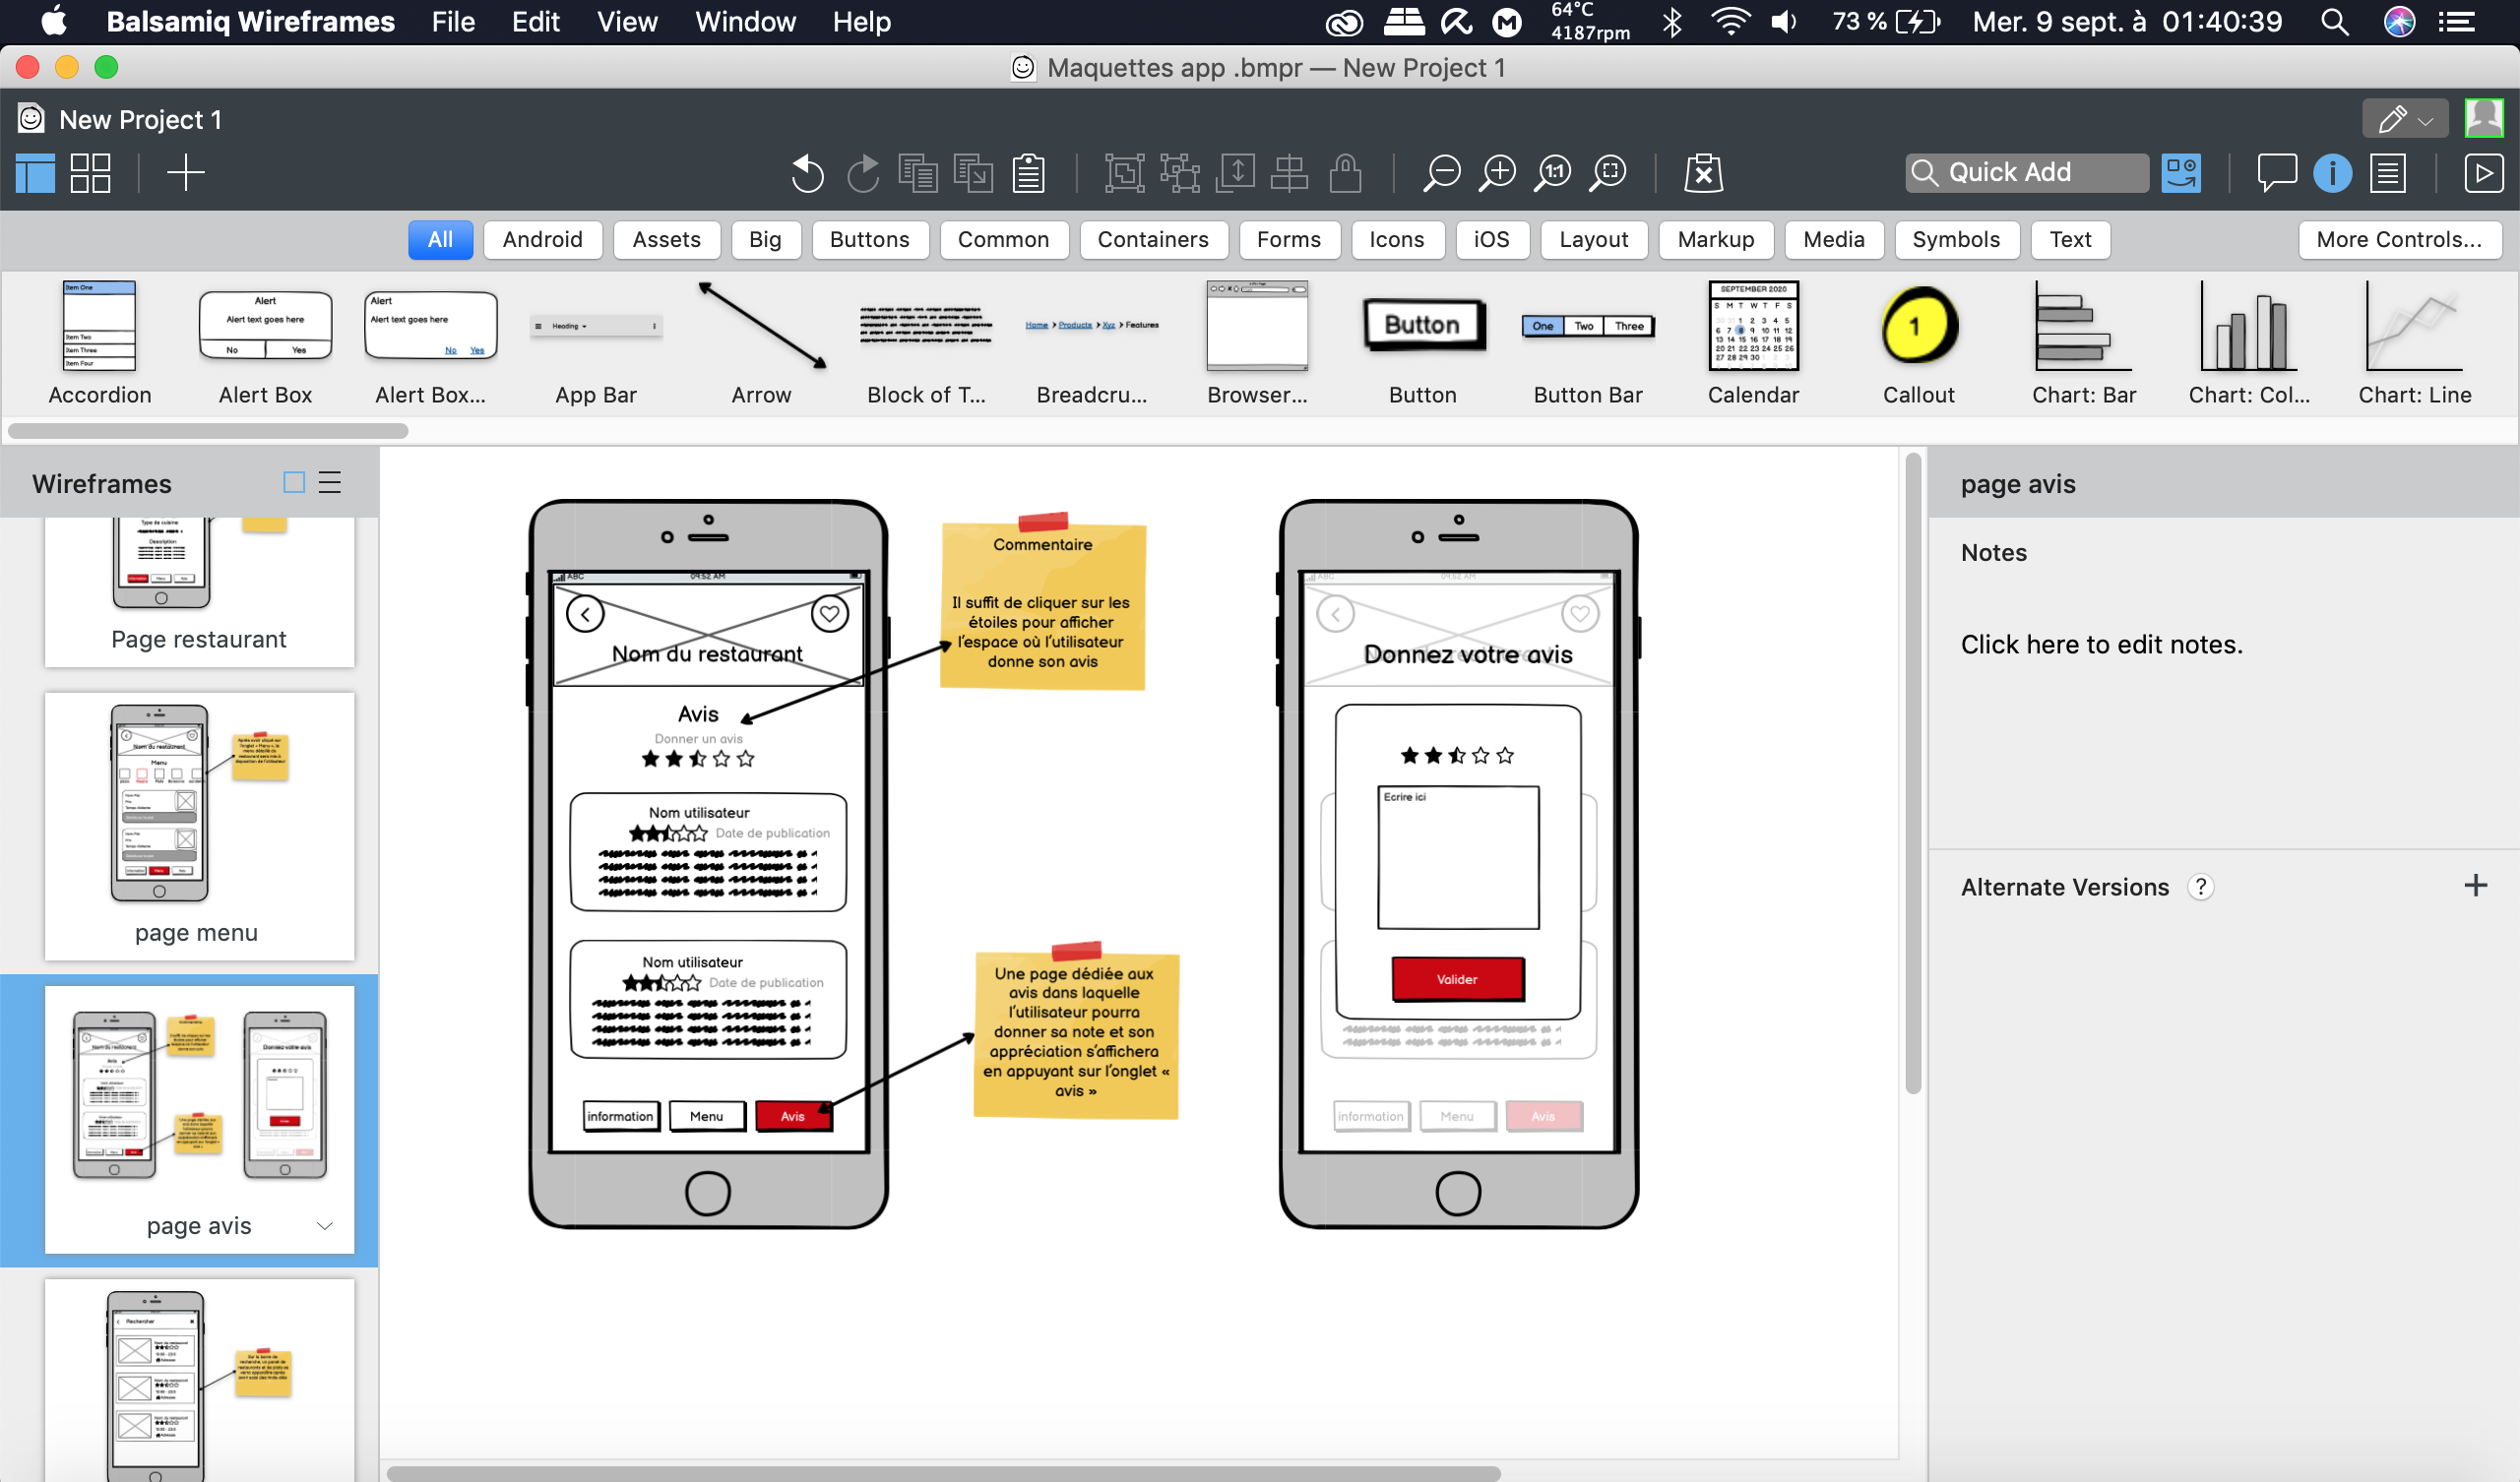
\includegraphics[width=6in]{images/Chapitre3/interface_balsamiq.png}
    \label{fig:interfacebalsamiq}
    \caption{Interface du logiciel Balsamiq}
\end{figure}
\newpage
\subsubsection{Les différents ecrans}
\begin{figure}[!h]
    \centering
    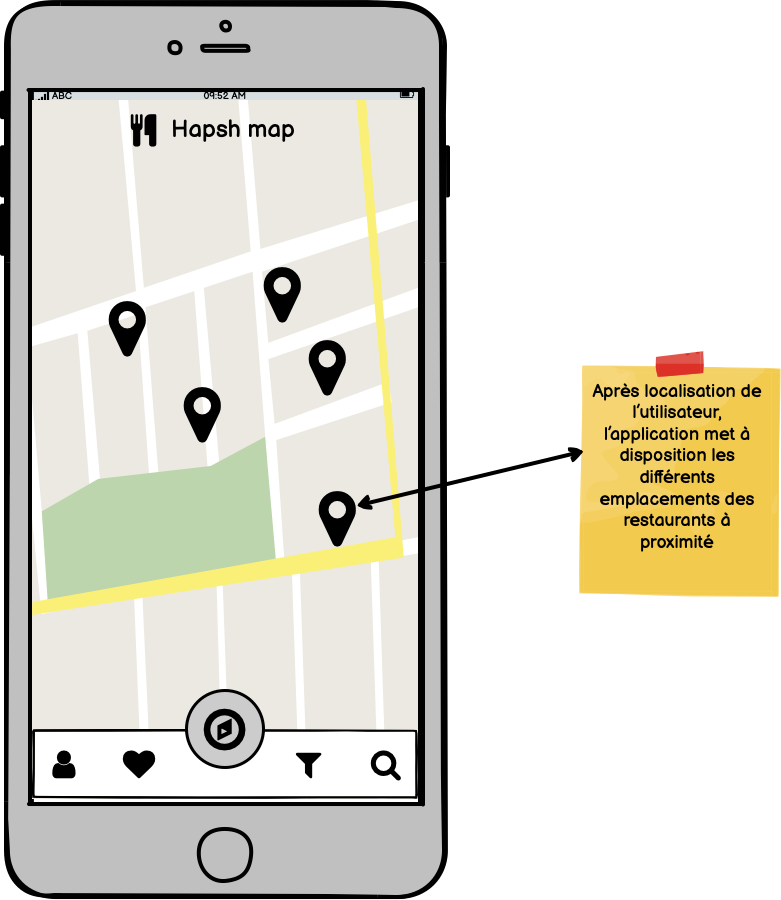
\includegraphics[width=8cm]{images/Chapitre3/maquettes_balsamiq/Acceuil.png}
    \label{fig:acceuil}
    \caption{Ecran principal}
\end{figure} 
\begin{figure}[!h]
    \centering
    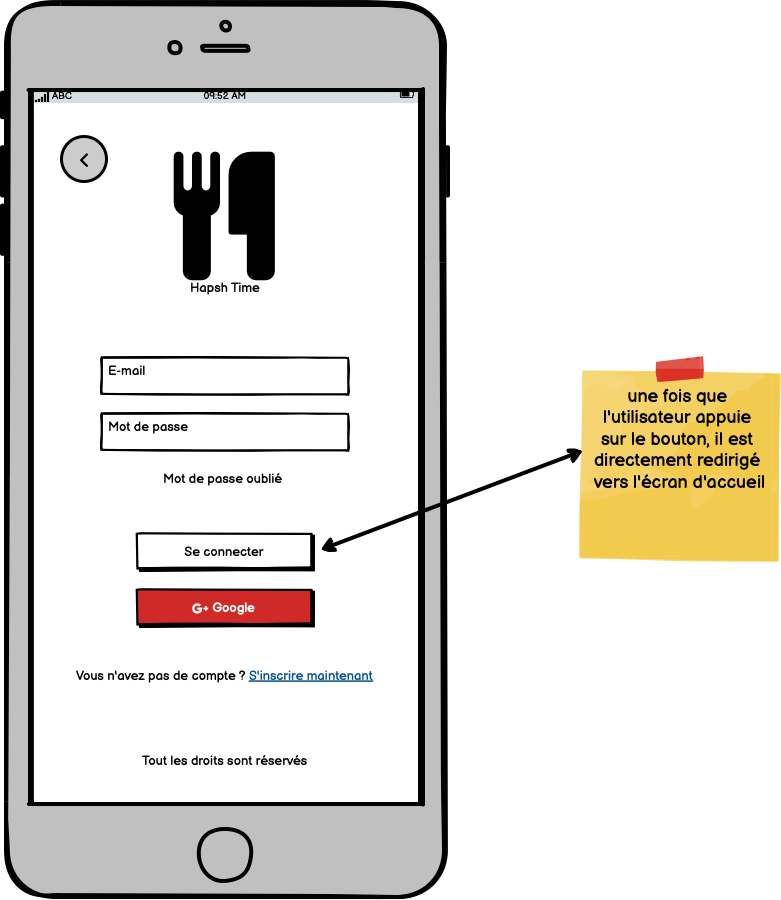
\includegraphics[width=8cm]{images/Chapitre3/maquettes_balsamiq/Connection.png}
    \label{fig:connexion}
    \caption{Ecran de connexion}
\end{figure} 
\newpage
\begin{figure}[!h]
    \centering
    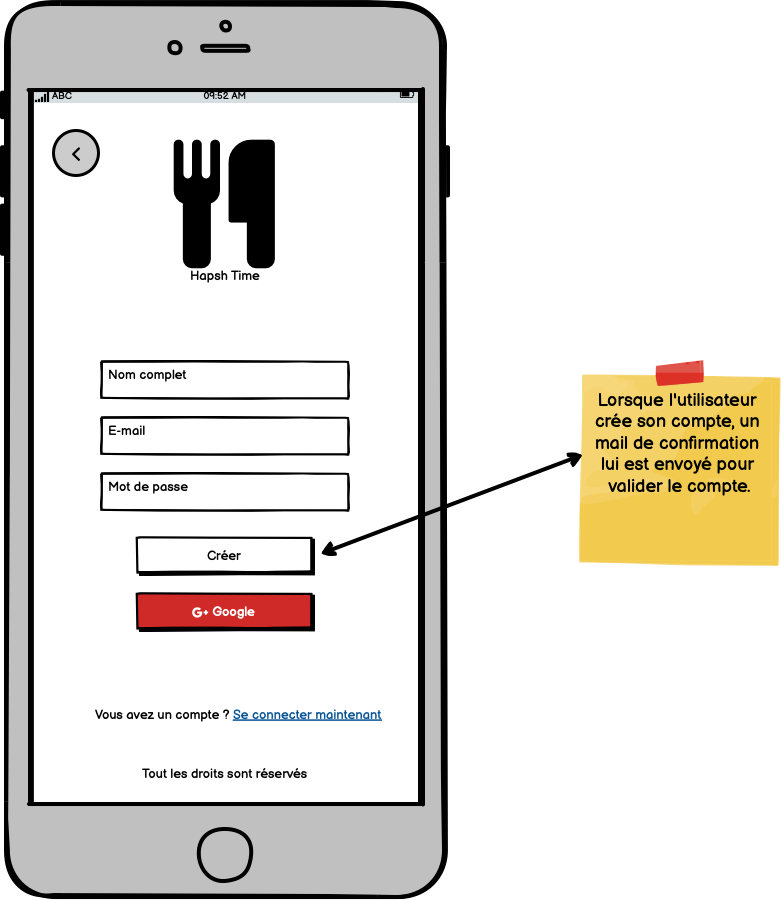
\includegraphics[width=8cm]{images/Chapitre3/maquettes_balsamiq/Creer.png}
    \label{fig:creation}
    \caption{Ecran de creation du compte}
\end{figure} 
\begin{figure}[!h]
    \centering
    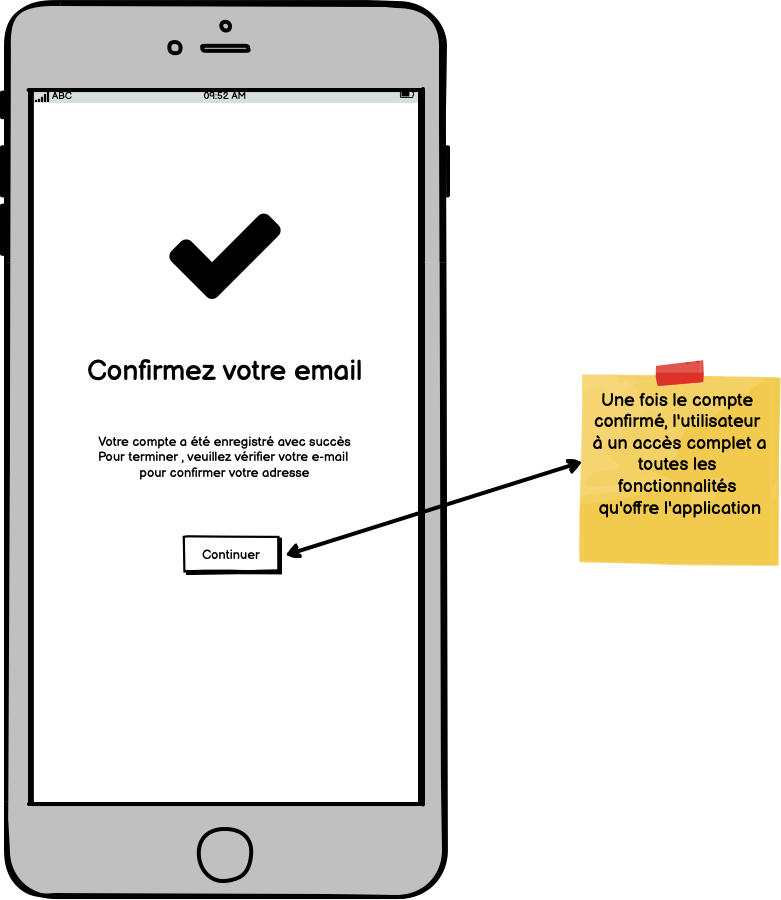
\includegraphics[width=8cm]{images/Chapitre3/maquettes_balsamiq/Confirmation.png}
    \label{fig:confirmation}
    \caption{Ecran de confirmation du compte}
\end{figure} 
\newpage
\begin{figure}[!h]
    \centering
    \includegraphics[width=8cm]{images/Chapitre3/maquettes_balsamiq/mot_de_passe_oublié.png}
    \label{fig:mdpoublié}
    \caption{Ecran de réinitialisation du mot de passe}
\end{figure} 
\begin{figure}[!h]
    \centering
    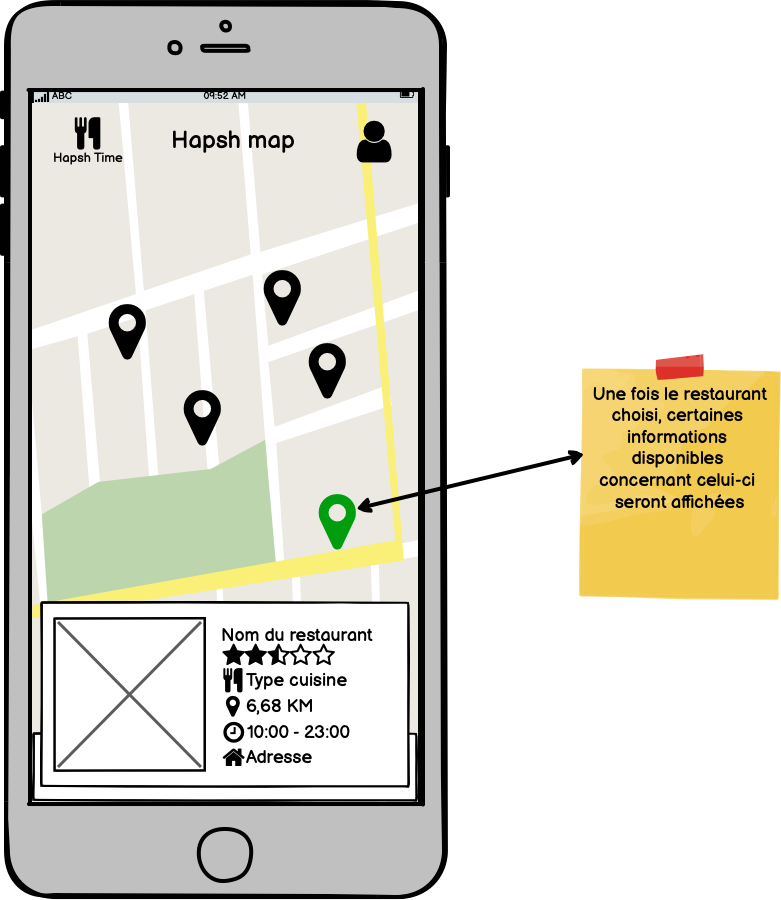
\includegraphics[width=8cm]{images/Chapitre3/maquettes_balsamiq/Restaurant_card.png}
    \label{fig:restocard}
    \caption{Ecran d'affichage de la fenêtre du restaurant}
\end{figure} 
\newpage
\begin{figure}[!h]
    \centering
    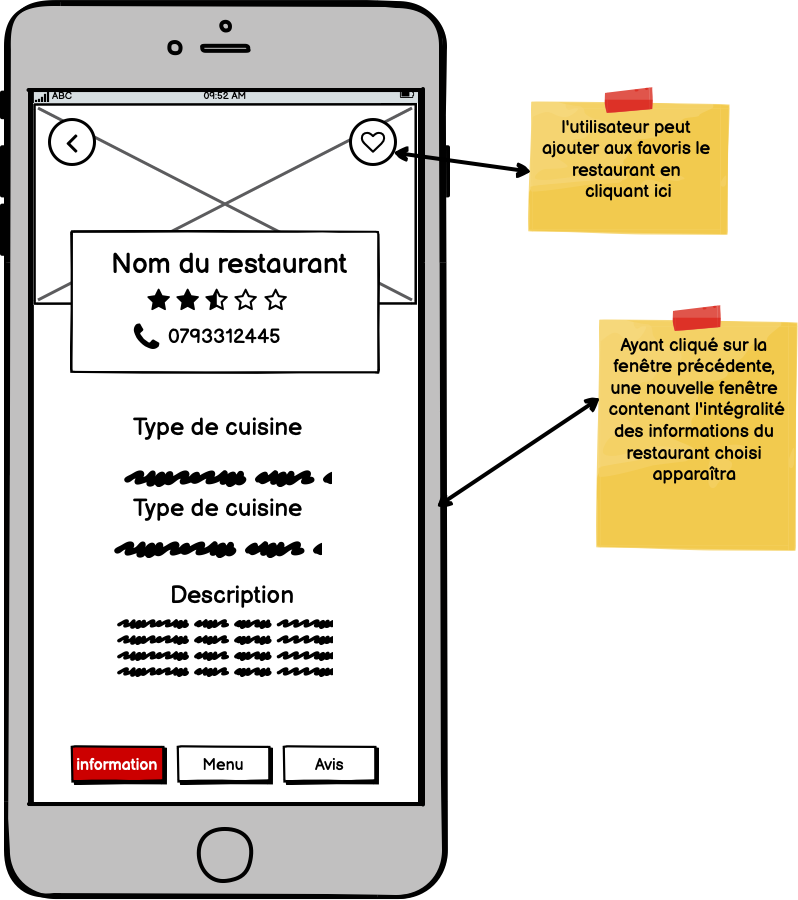
\includegraphics[width=8cm]{images/Chapitre3/maquettes_balsamiq/Page_restaurant.png}
    \label{fig:pageresto}
    \caption{Page de détails du restaurant}
\end{figure} 
\begin{figure}[!h]
    \centering
    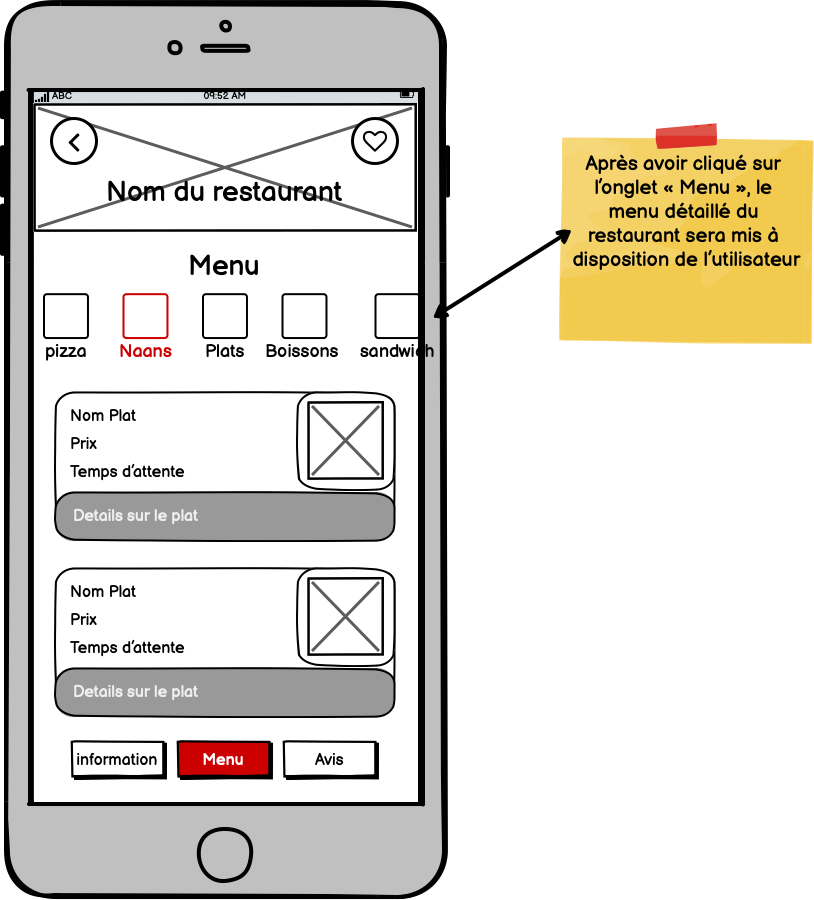
\includegraphics[width=8cm]{images/Chapitre3/maquettes_balsamiq/page_menu .png}
    \label{fig:pagemenu}
    \caption{Page de détails du menu}
\end{figure} 
\newpage
\begin{figure}[!h]
    \centering
    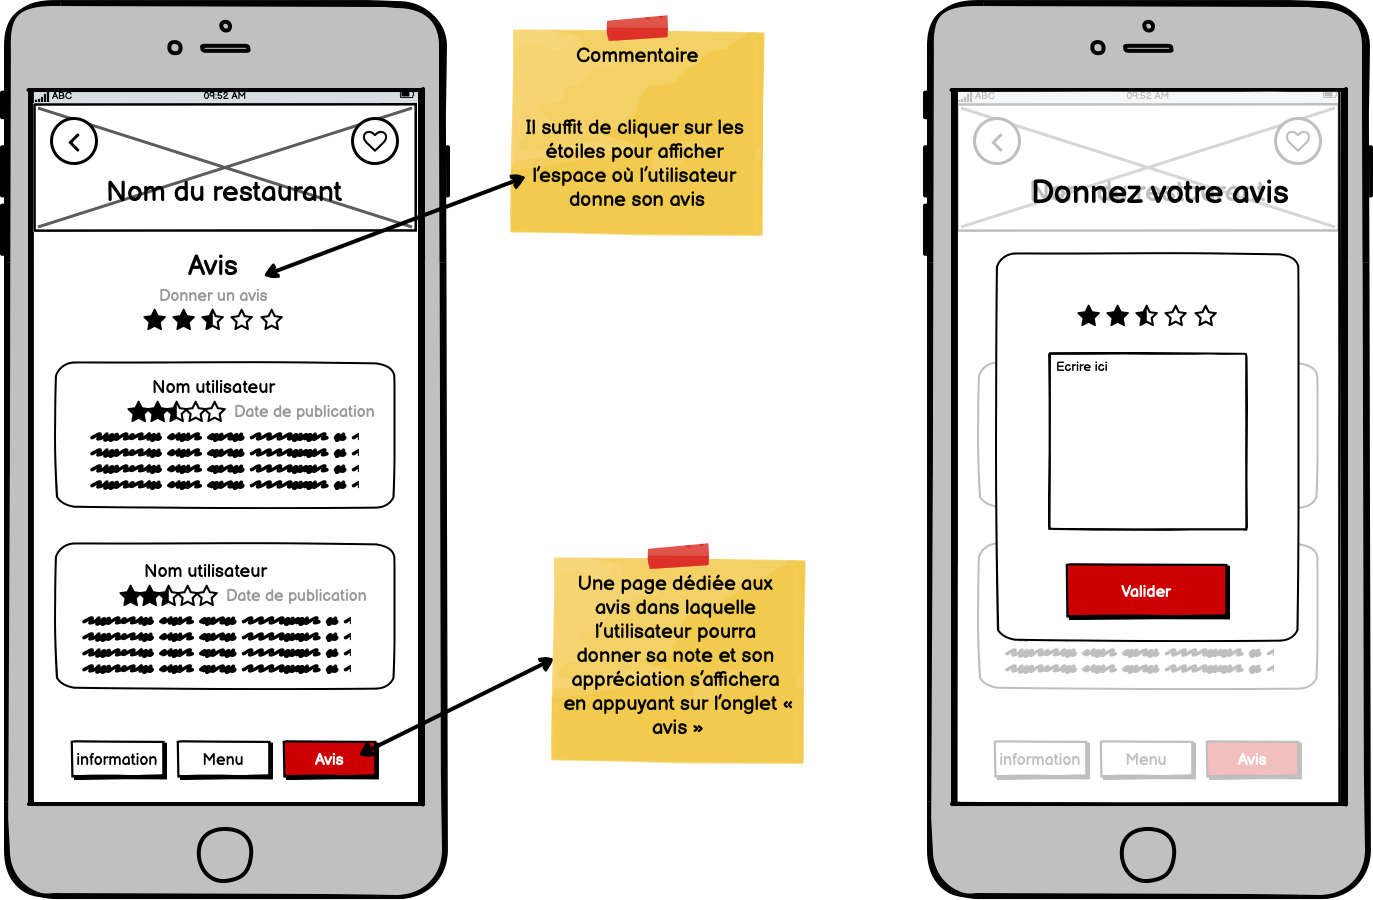
\includegraphics[width=14cm]{images/Chapitre3/maquettes_balsamiq/page_avis.png}
    \label{fig:pageavis}
    \caption{Page d'avis}
\end{figure} 
\begin{figure}[!h]
    \centering
    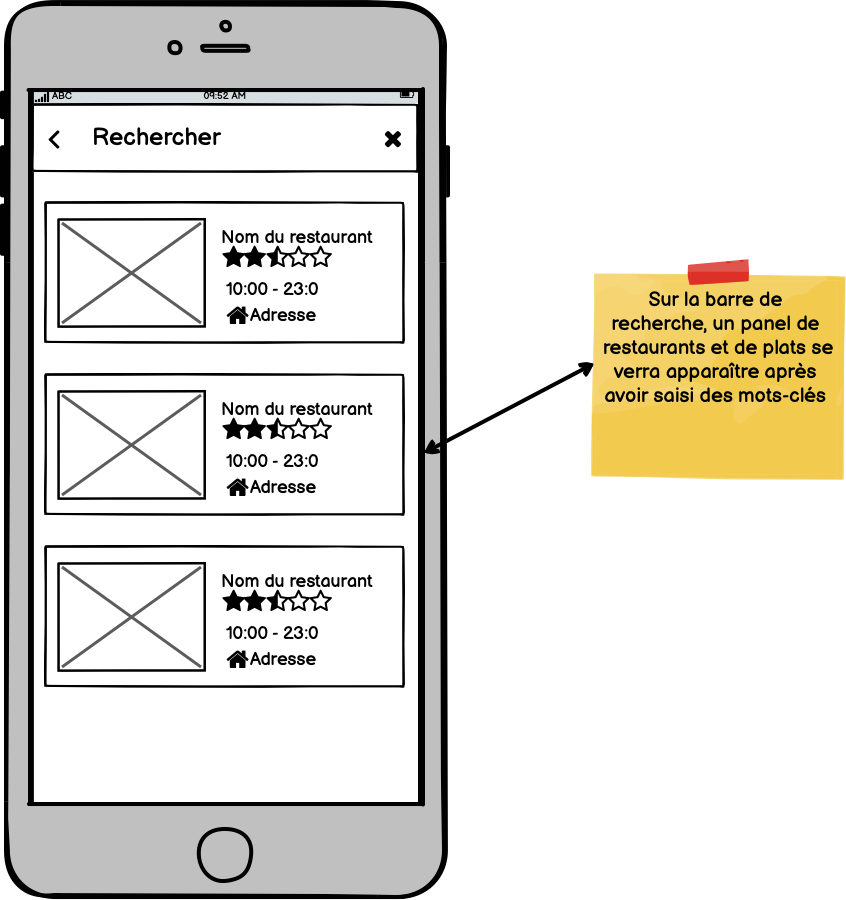
\includegraphics[width=8cm]{images/Chapitre3/maquettes_balsamiq/Page_de_recherche.png}
    \label{fig:pagerecherche}
    \caption{Page de recherche}
\end{figure} 
\newpage
\begin{figure}[!h]
    \centering
    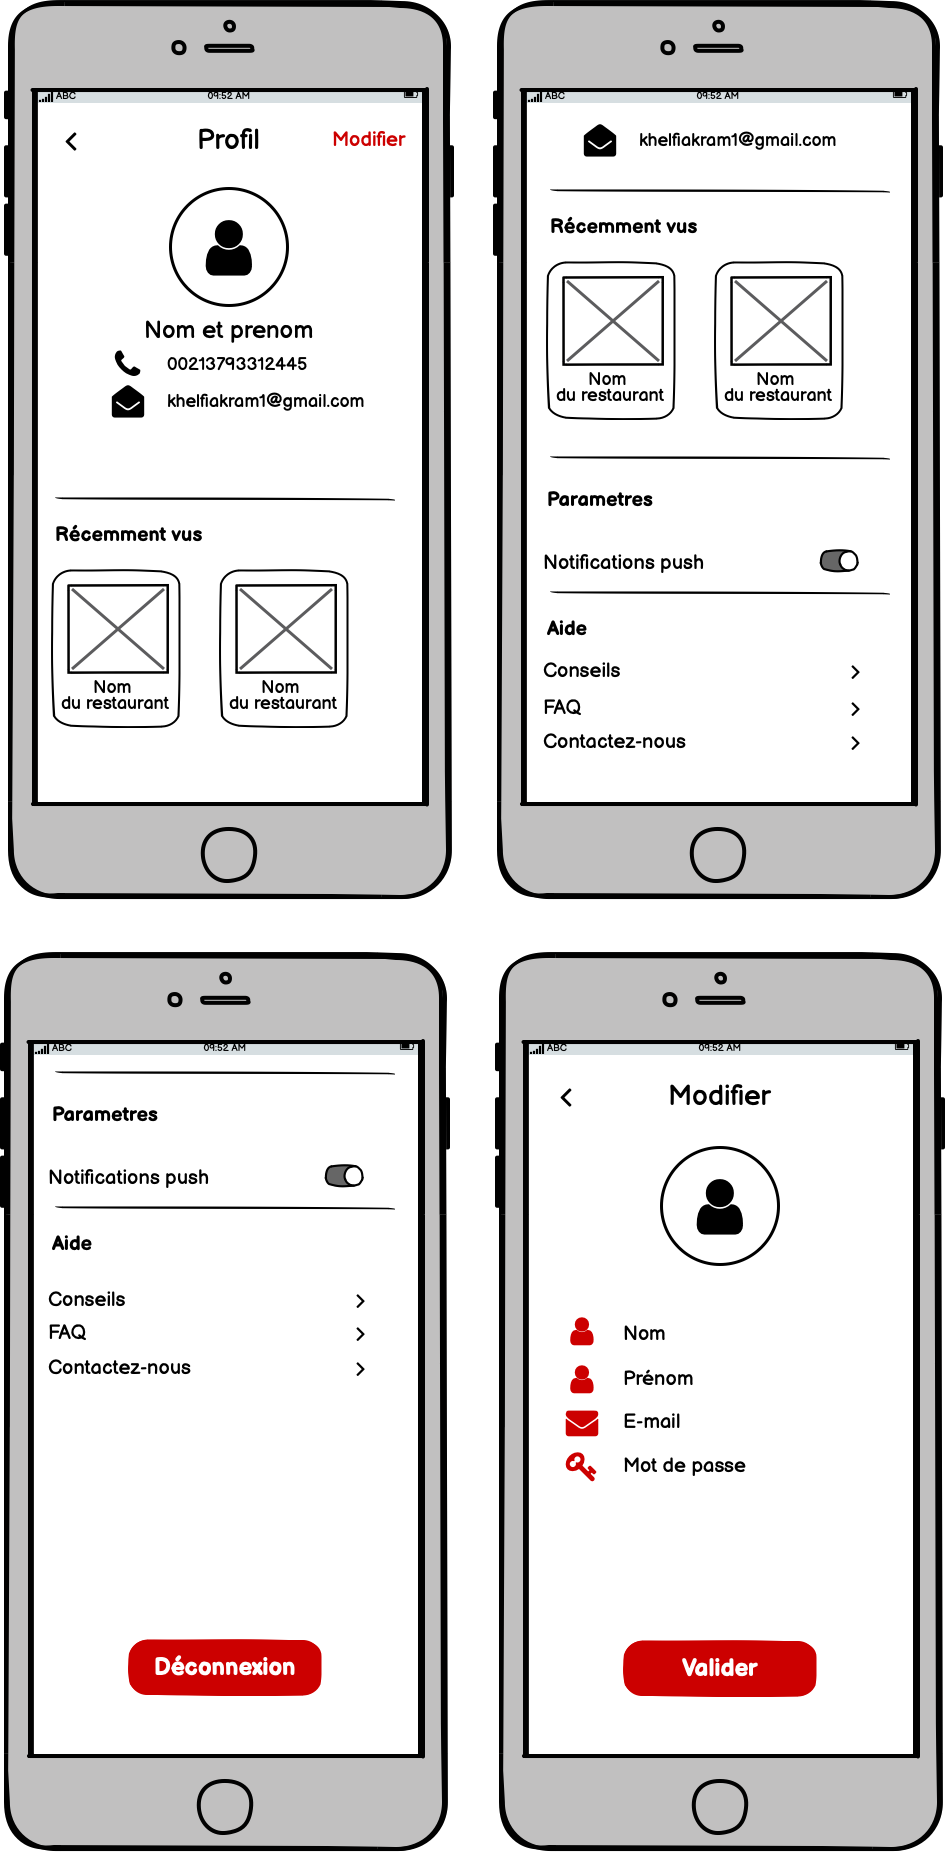
\includegraphics[width=10cm]{images/Chapitre3/maquettes_balsamiq/Profil.png}
    \label{fig:profil}
    \caption{Page du profil et parametres}
\end{figure} 
\newpage
\begin{figure}[!h]
    \centering
    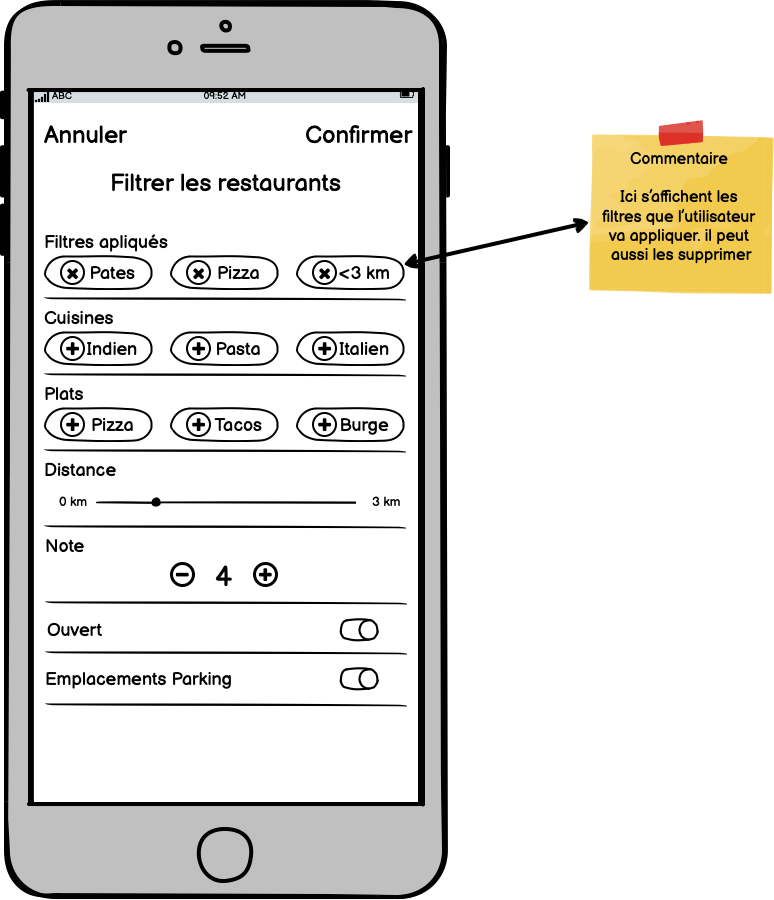
\includegraphics[width=8cm]{images/Chapitre3/maquettes_balsamiq/Filtre.png}
    \label{fig:filtre}
    \caption{Page du filtre}
\end{figure} 
\begin{figure}[!h]
    \centering
    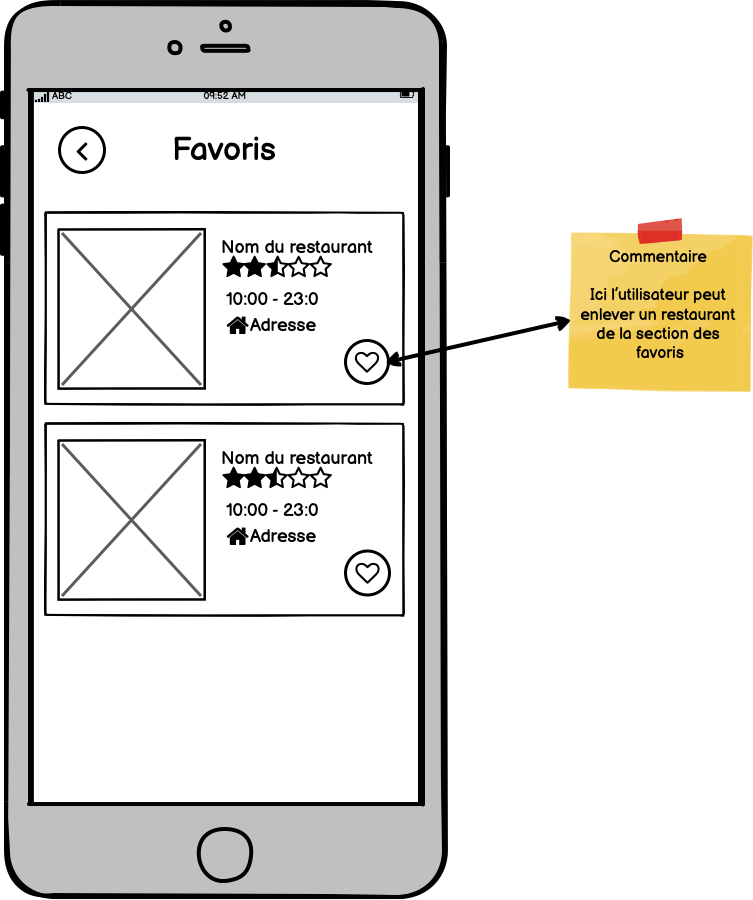
\includegraphics[width=8cm]{images/Chapitre3/maquettes_balsamiq/favorite_restaurants.png}
    \label{fig:favoris}
    \caption{Page des restaurants favoris}
\end{figure} 
\newpage
\subsection{Prototypage et interface utilisateur}
La phase de Prototypage et de la création de l'interface utilisateur est une étape très importante dans le développement des applications mobiles. pour ce projet on a utilisé les règles de design appelées le material design de Google qui est un design très présent dans les applications mobiles en ce temps.
\subsubsection{Material design}
Le Material Design est un ensemble de règles de design proposées par Google et qui s'appliquent a l'interface graphique 
des logiciels et applications . Il est utilisé notamment a partir de la verison 5.0 (Lolipop) du systéme d'exploitation 
Android.

Google a présenté le Material Design pour la première fois lors de la conférence Google I/O, le 25 juin 2014. Ces régles 
de design mettent l'accent sur une utilisation accrue des mises en page basées sur une grille , des animations et des
transitions, des effets de profondeur tels l'éclairage et les ombres. Selon Google ce nouveau language de design est basé 
sur le papier et l'encre.

Le designer Matías Duarte explique que « contrairement au vrai papier, notre matériau numérique peut s'étirer et se 
modifier de manière intelligente. Le matériau contextuel a une surface physique et des bords. Les superpositions et 
les ombres donnent des informations sur ce que vous pouvez toucher ».~\cite{MaterialDesign2020}
\begin{figure}[!h]

    \centering
    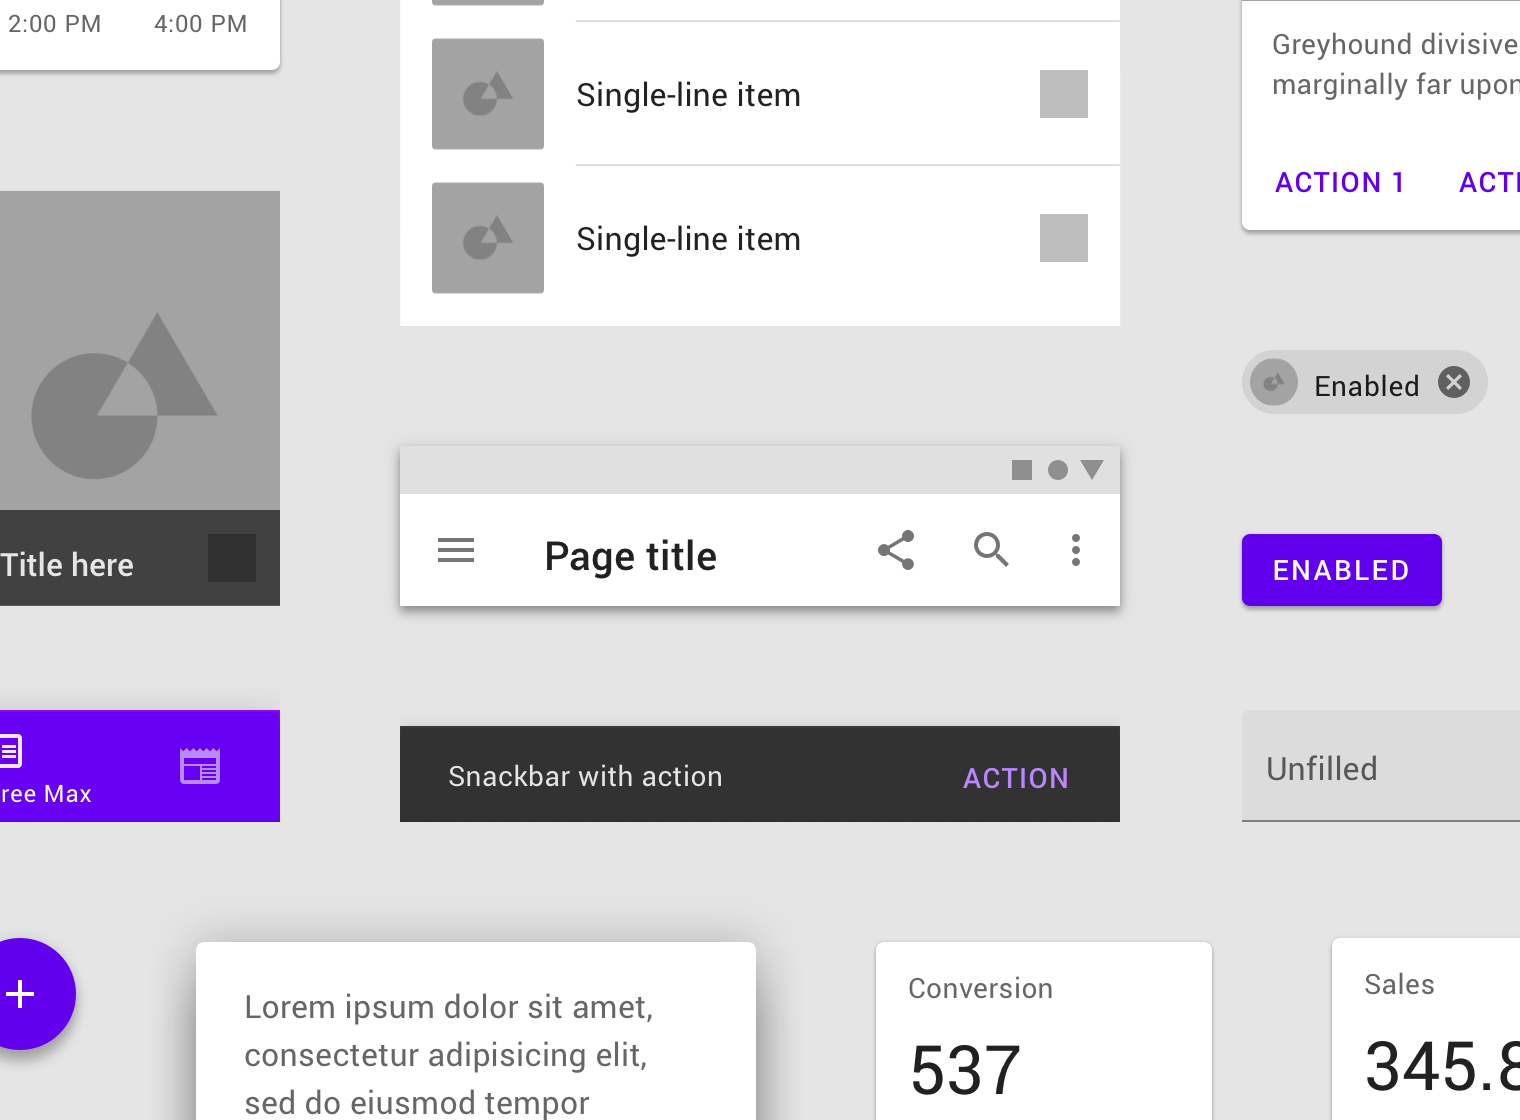
\includegraphics[width=5in]{images/Chapitre3/material design.png}
    \label{fig:label5}
    \caption{Exemple de composantes du Material Design}
\end{figure}
\subsubsection{Outil utilisé (Adobe XD)}
Adobe XD est unoutil de conception de l' expérience utilisateur pour les applications Web et des applications mobiles , développé et édité par Adobe Inc . Il est disponible pour macOS et Windows , bien qu'il existe des versions pour iOS et Android pour aider à prévisualiser le résultat du travail directement sur les appareils mobiles. XD prend en charge le wireframing de site Web et la création de prototypes de clic ~\cite{AdobeXD2020}.
\begin{figure}[!h]

    \centering
    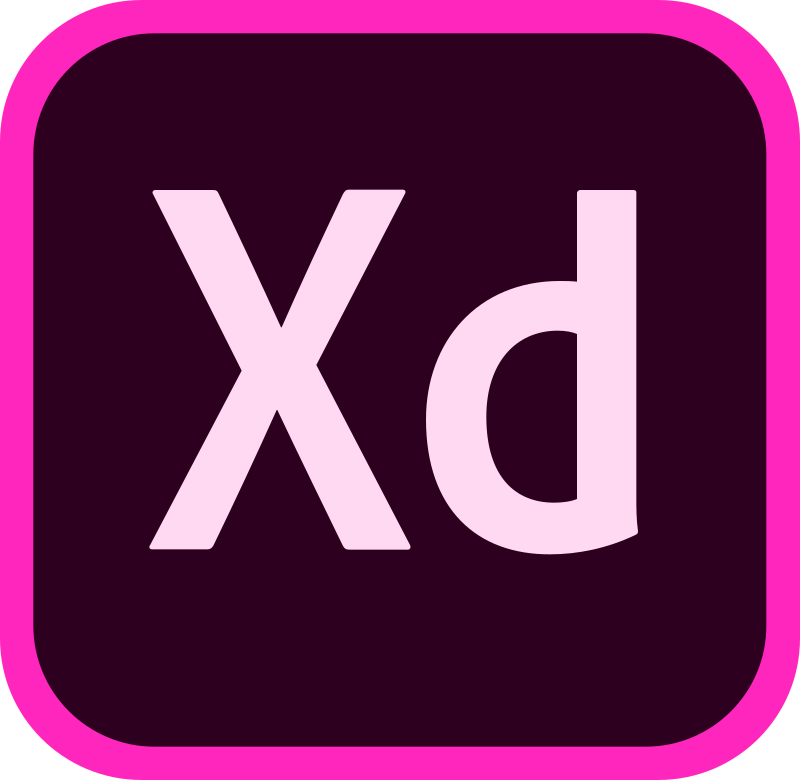
\includegraphics[width=3cm]{images/Chapitre3/AdobeXD.png}
    \label{fig:label6}
    \caption{Logo de Adobe XD}
\end{figure}
\begin{figure}[!h]

    \centering
    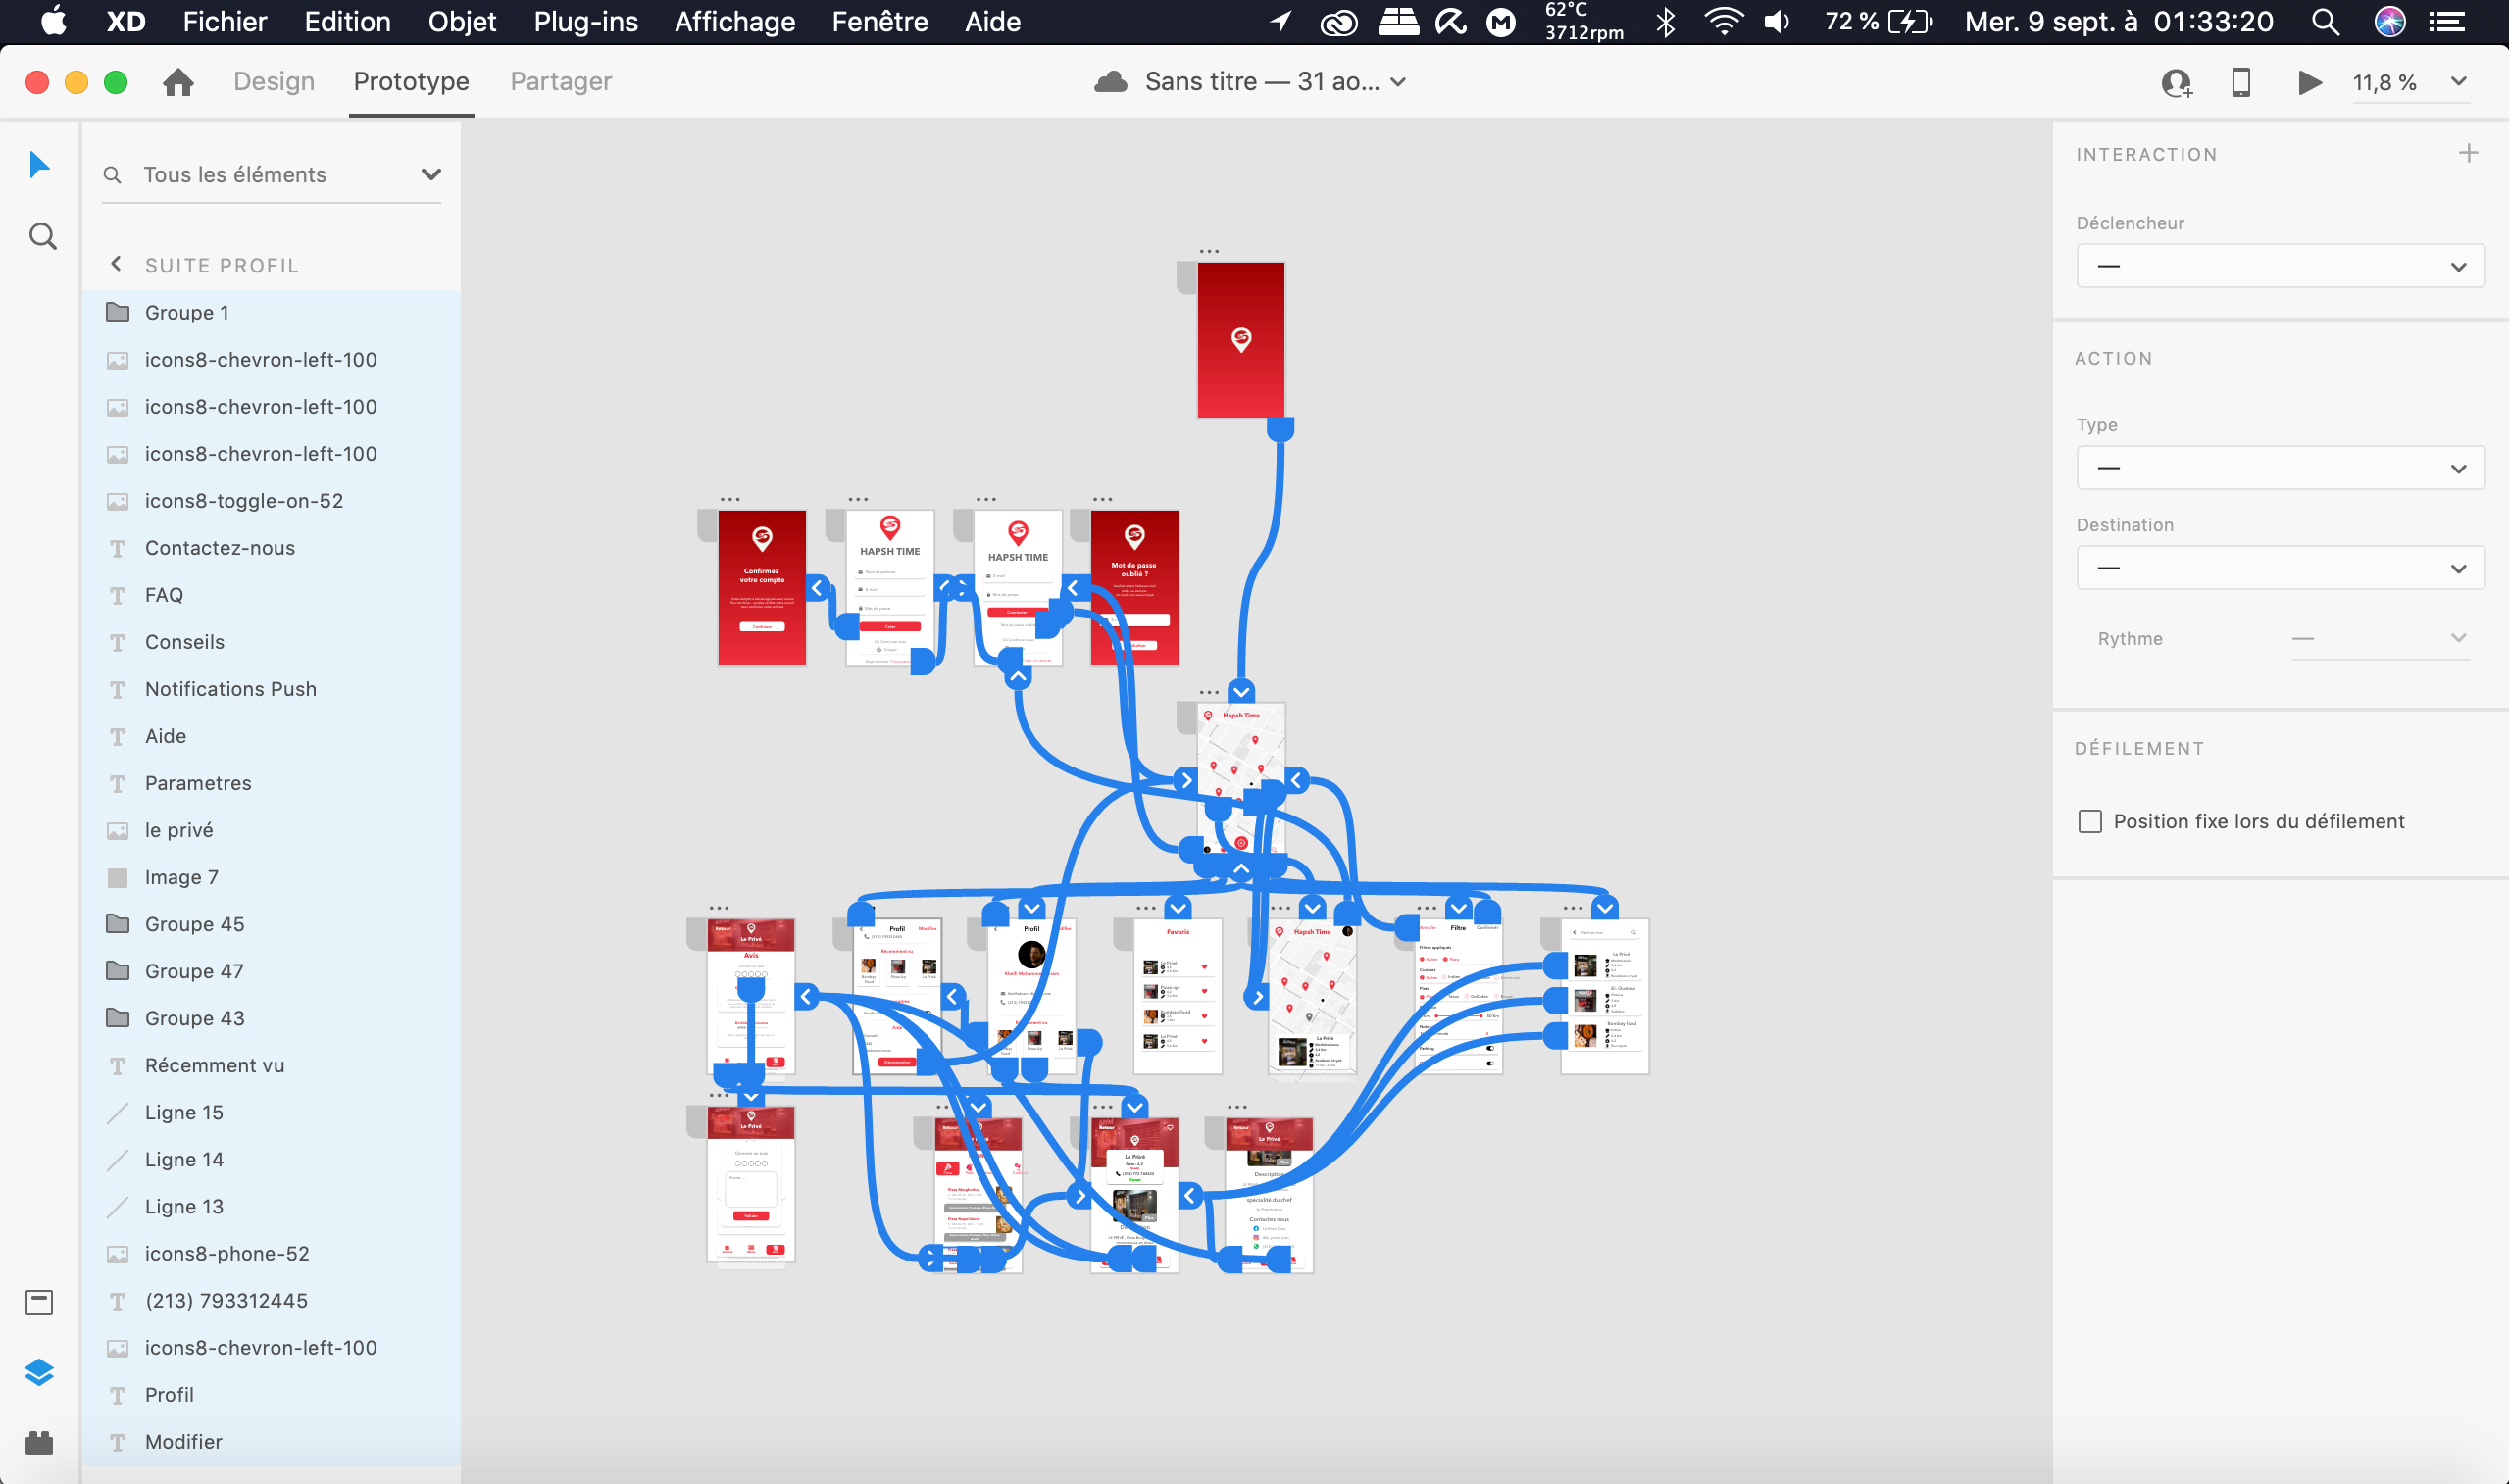
\includegraphics[width=6.5in]{images/Chapitre3/interface_adobe_xd.png}
    \label{fig:label6}
    \caption{interface du logiciel Adobe XD}
\end{figure}

\newpage
\subsubsection{Les Maquettes UI/UX}
\begin{figure}[!h]

    \centering
    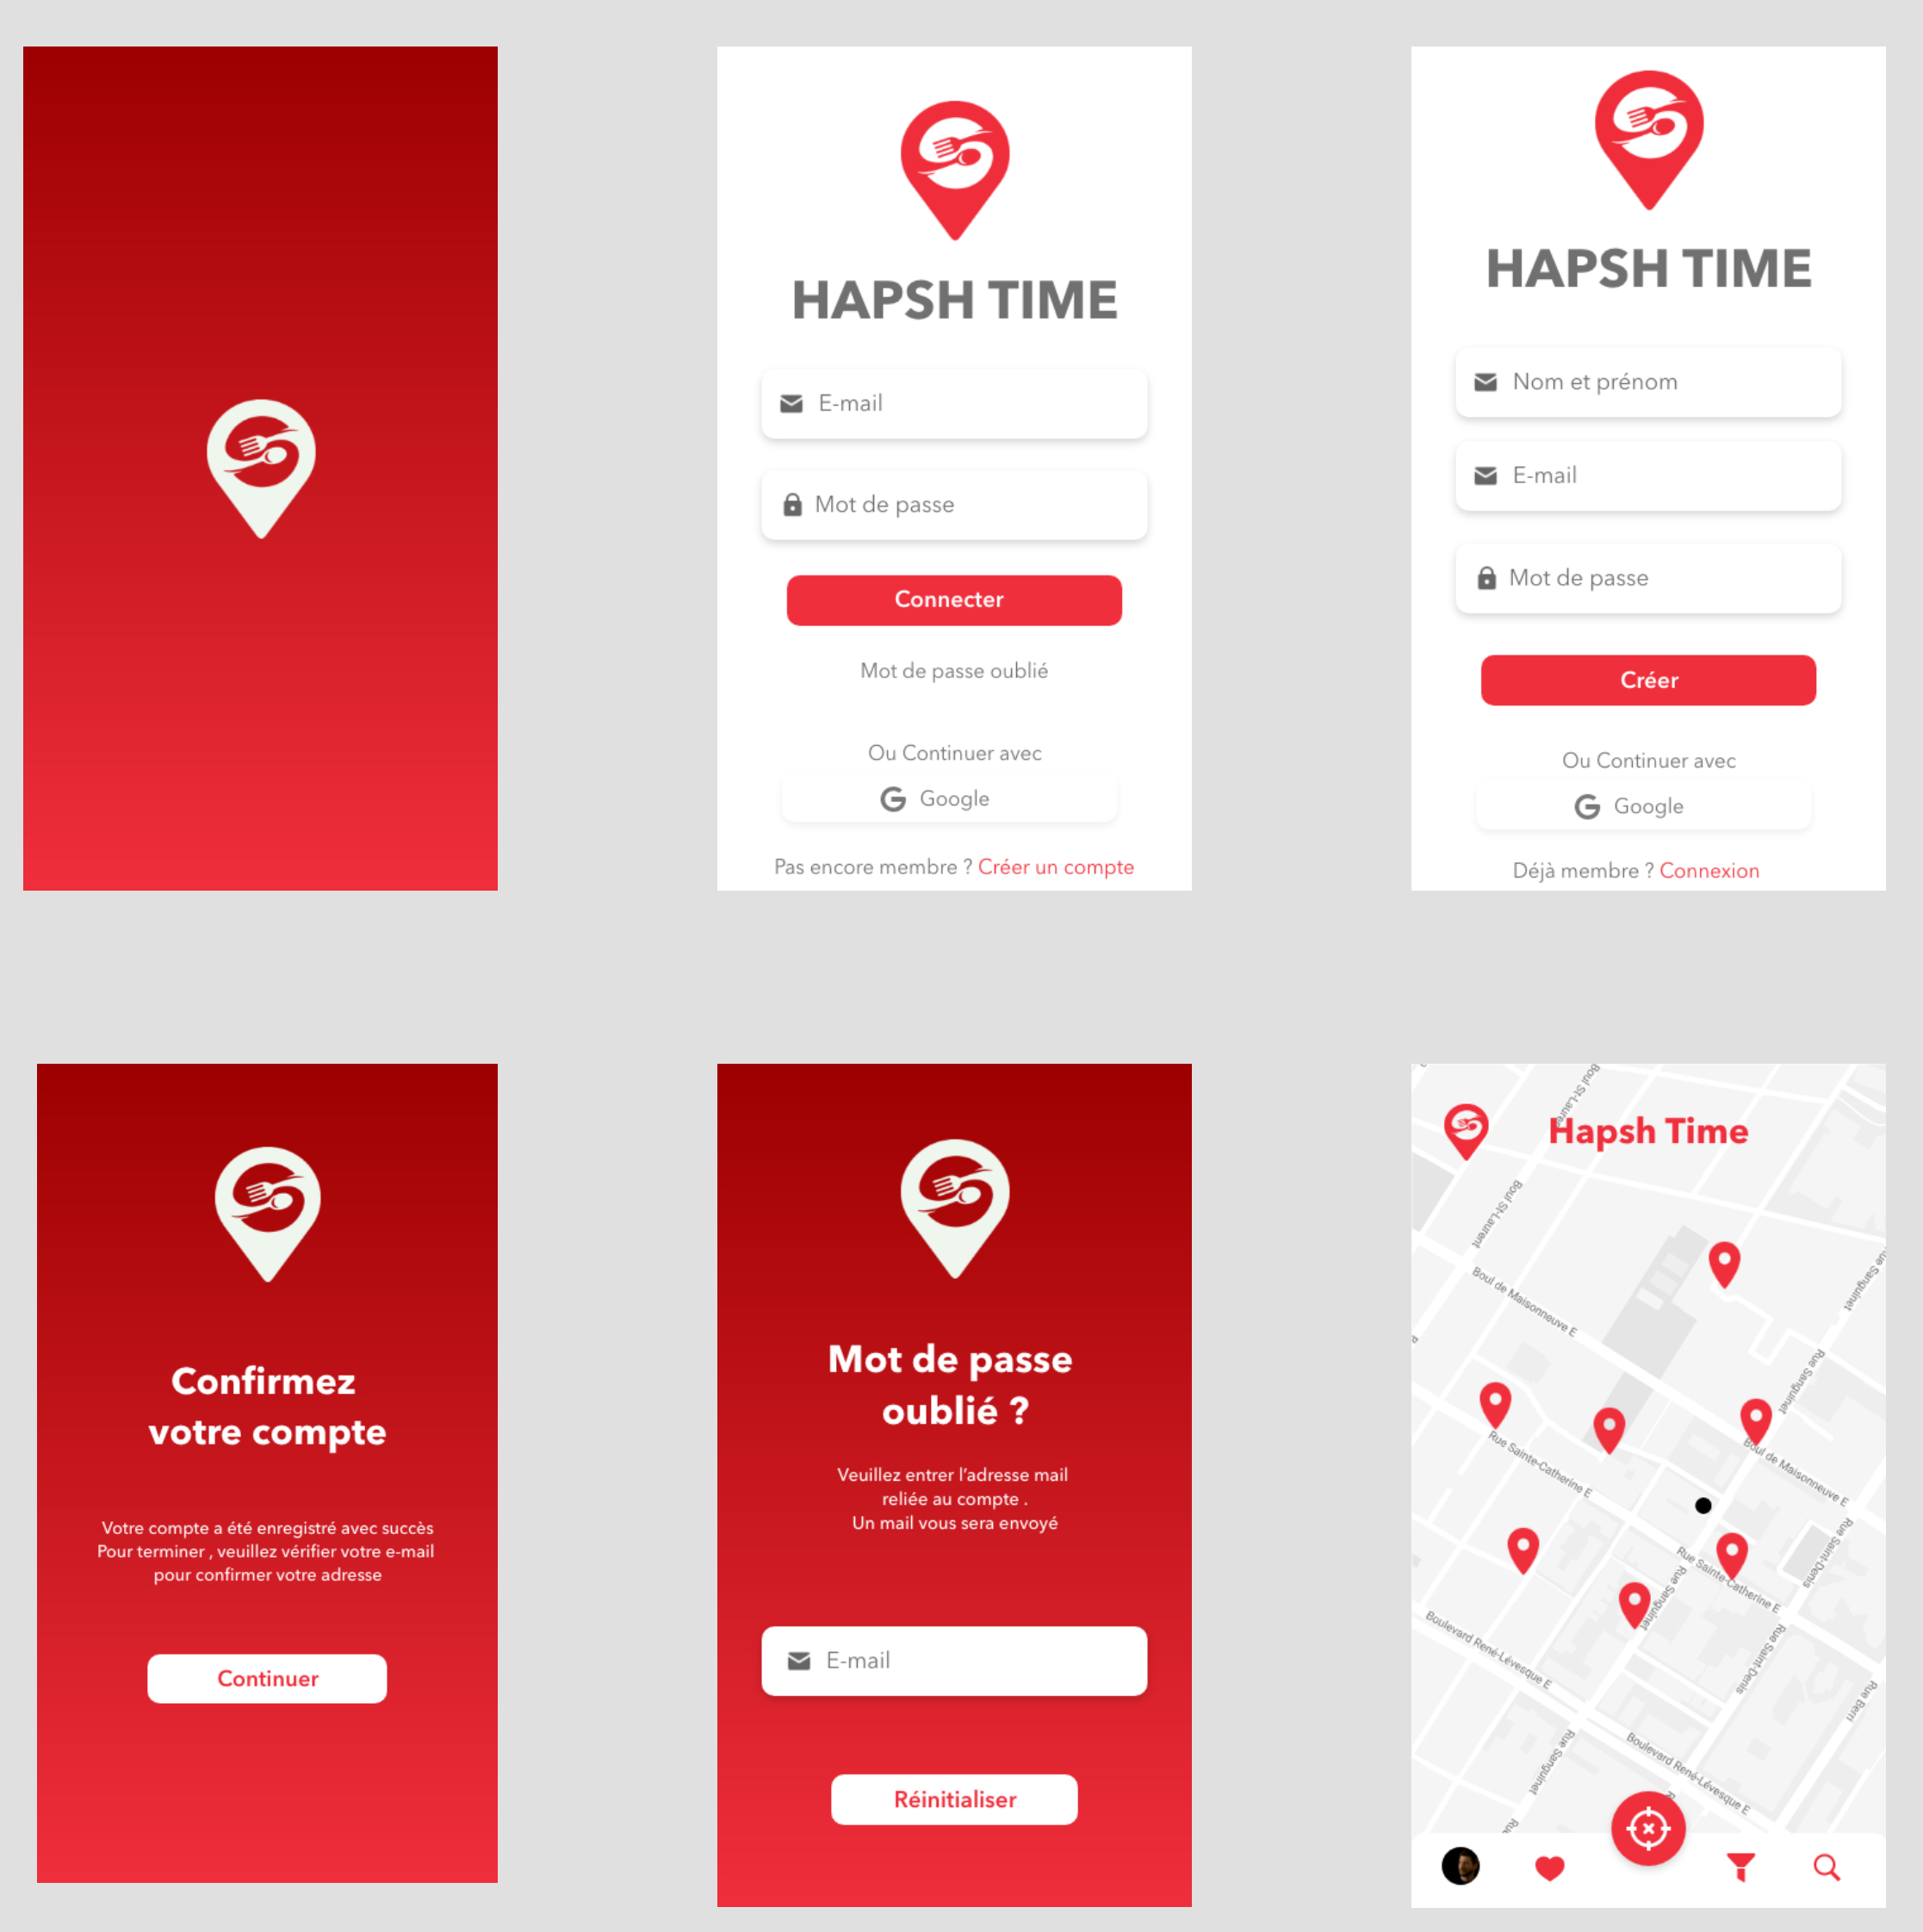
\includegraphics[width=6.5in]{images/Chapitre3/maquettes_balsamiq/p1.jpg}
    \label{fig:ux1}
   
\end{figure}
\newpage
\begin{figure}[!h]

    \centering
    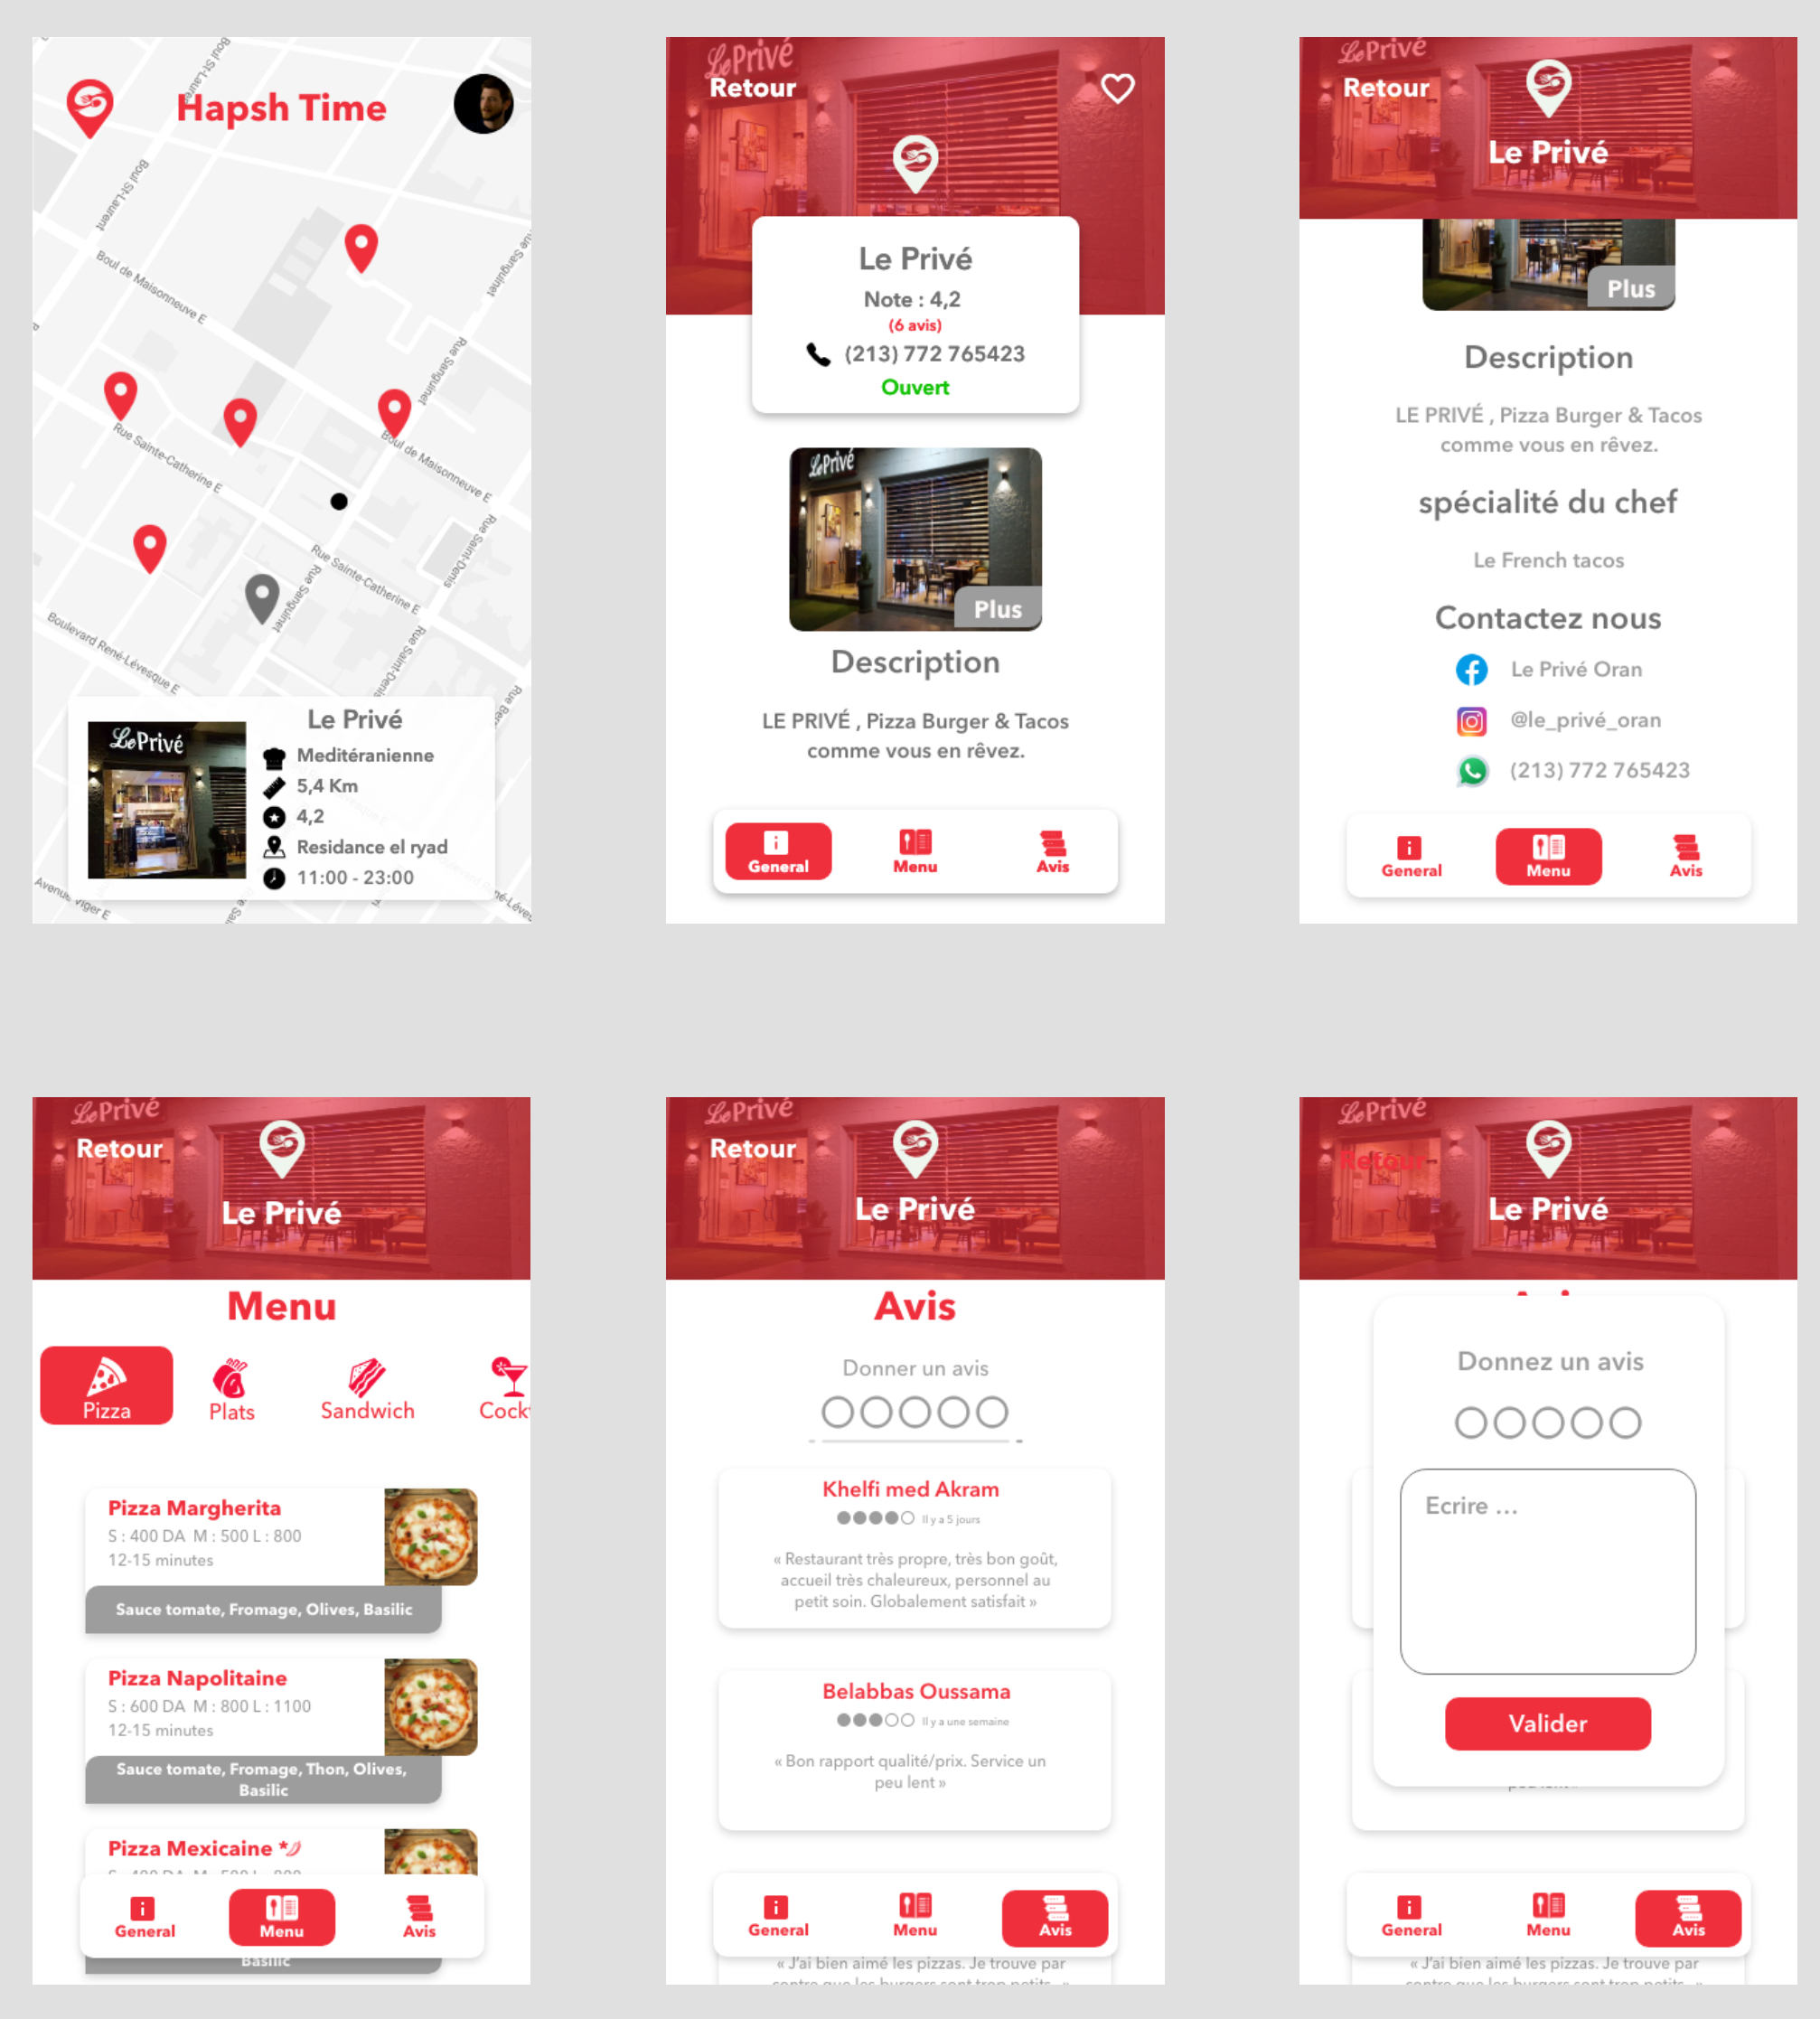
\includegraphics[width=6.5in]{images/Chapitre3/maquettes_balsamiq/p2.jpg}
    \label{fig:ux2}
   
\end{figure}
\newpage
\begin{figure}[!h]

    \centering
    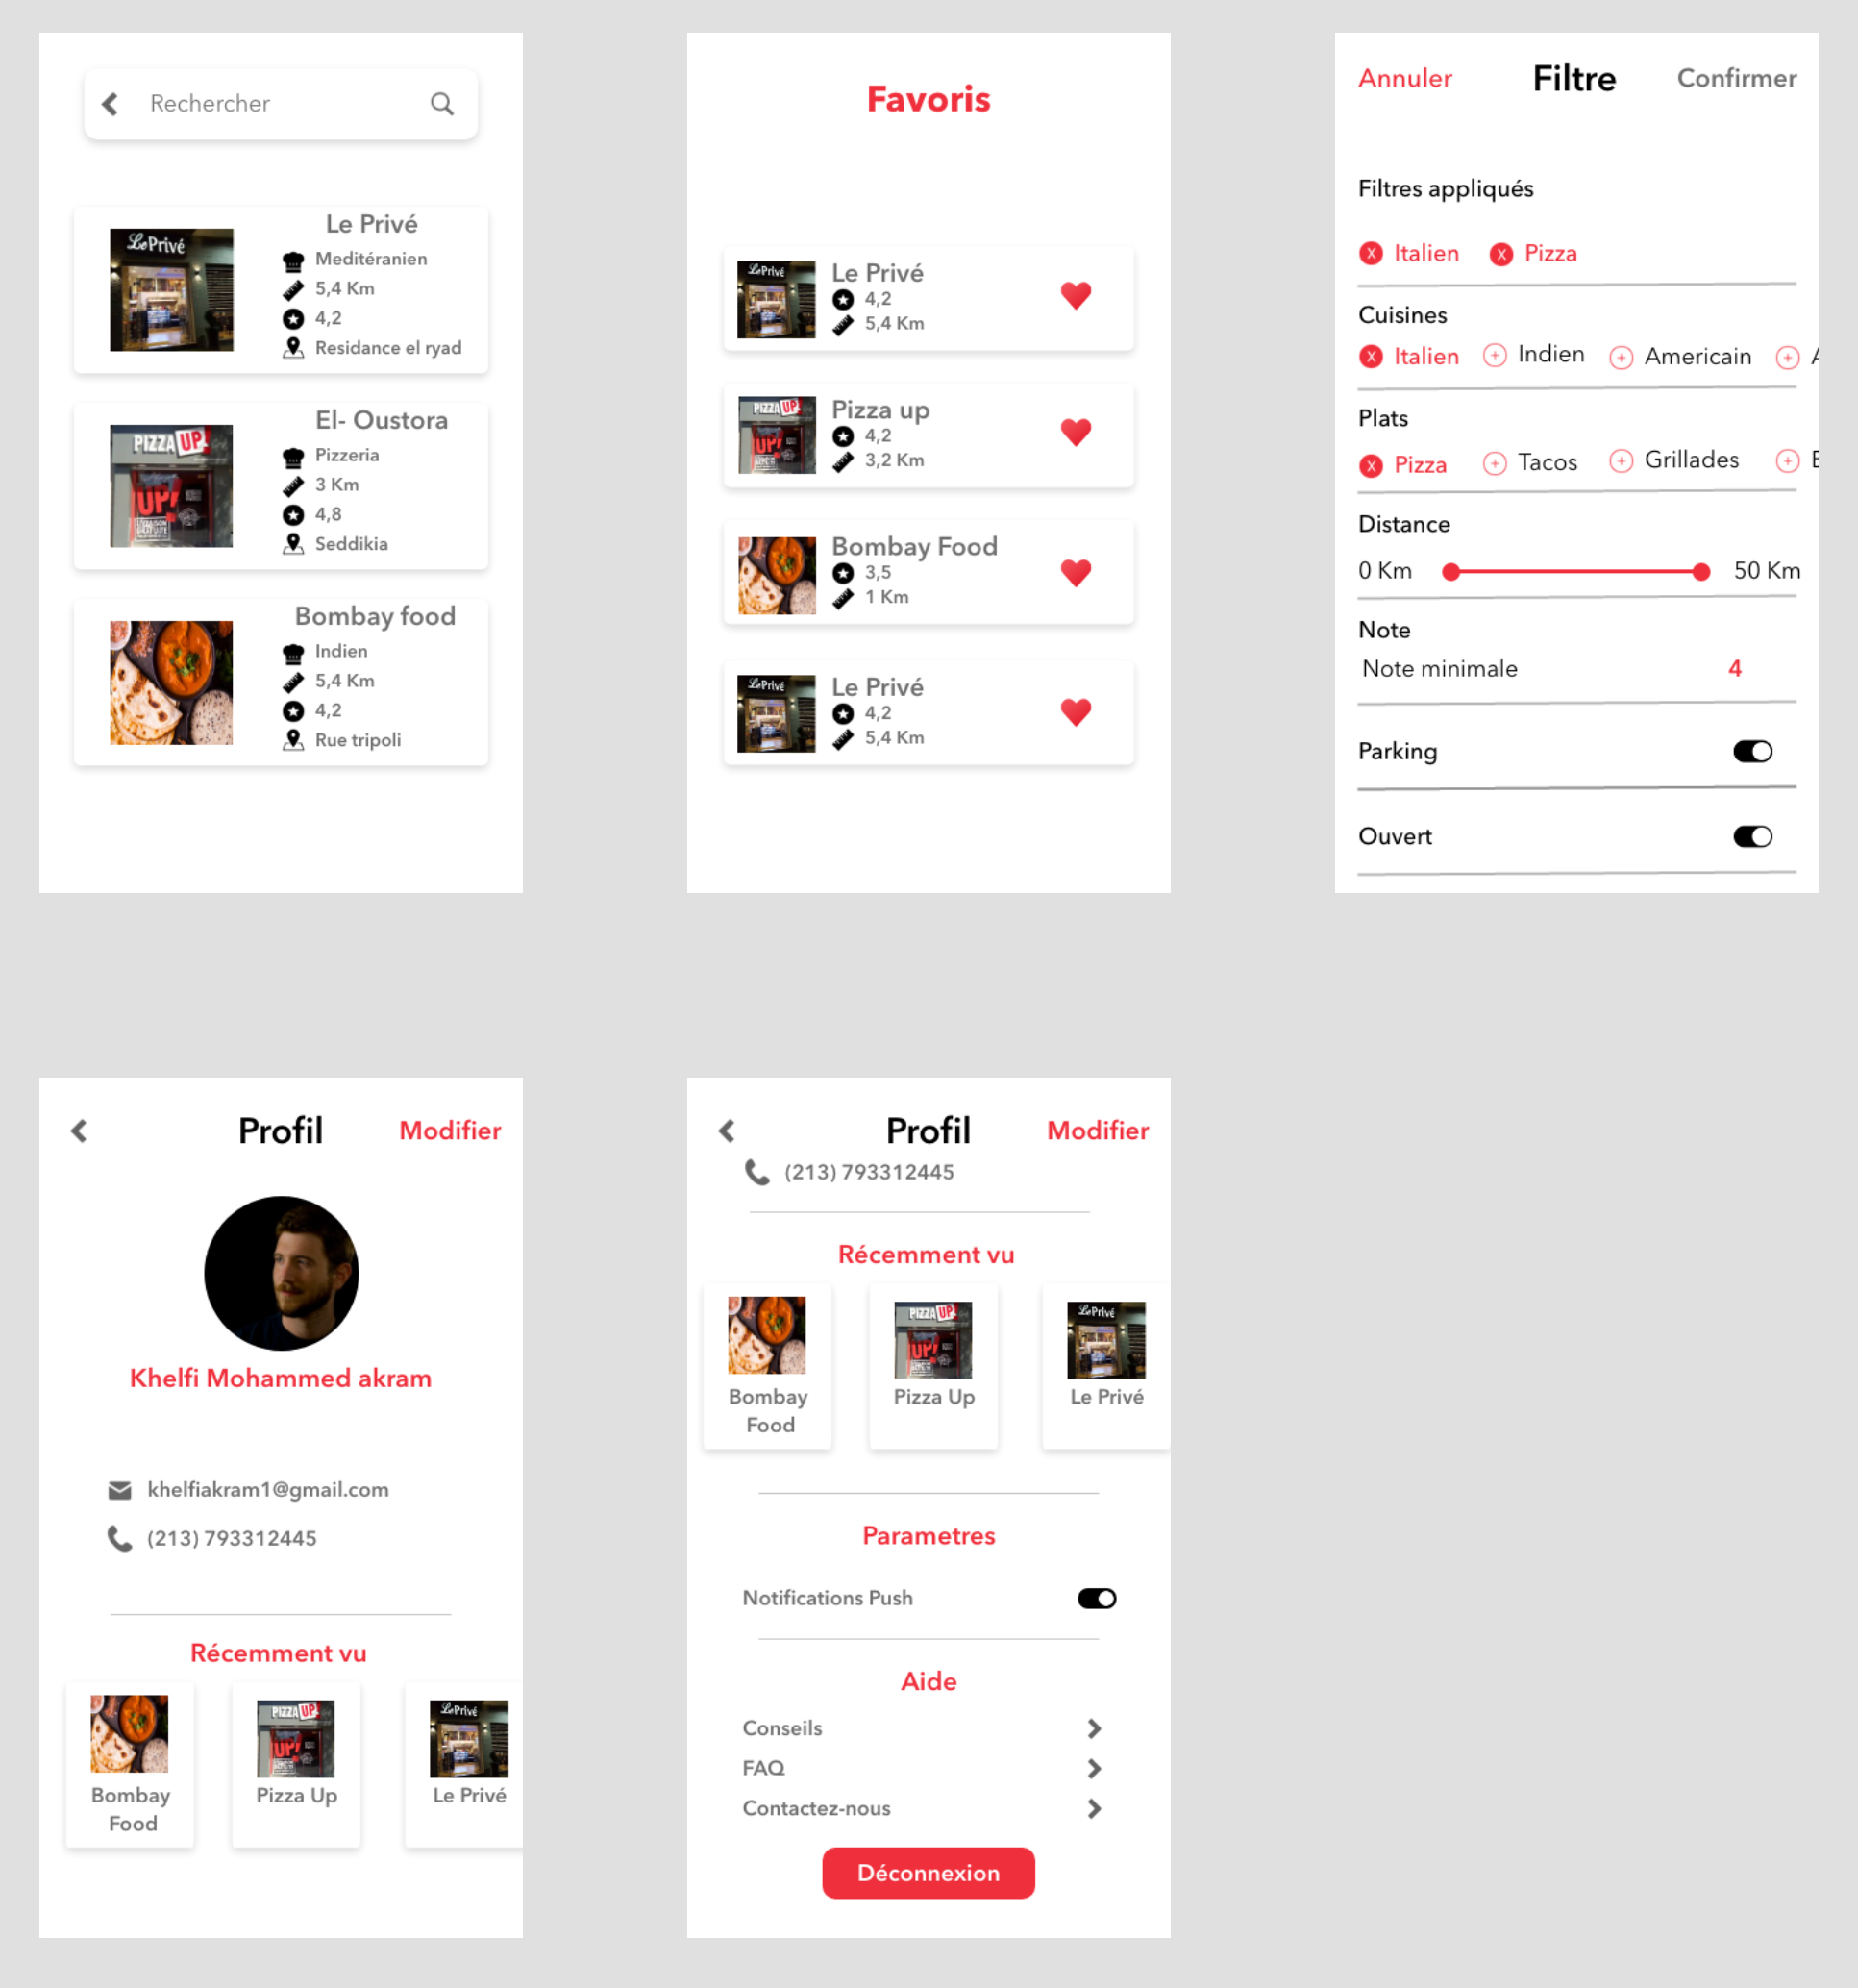
\includegraphics[width=6.5in]{images/Chapitre3/maquettes_balsamiq/p3.jpg}
    \caption{Interfaces utilisateur de l'application}

    \label{fig:ux3}
   
\end{figure}
\newpage
\section{Implementation}
\subsection{Outils Materiels}
Le développement de cette application a ete effectue sur deux machines en parallèle avec les configurations suivantes :
\\
\textbf{Machine principale}

\begin{itemize}
    \item Marque : Lenovo Thinkpad
    \item Syeteme d'exploitation : Windows 10
    \item Microprocesseur : Intel Core i5
    \item Mémoire vice : 8 Go
    \item Disque dur : 256 GO SSD
          
\end{itemize}
\textbf{Machine secondaire}
\begin{itemize}
    \item Marque : Dell .
    \item Syeteme d'exploitation : Ubuntu 19.10.
    \item Microprocesseur : Intel Core i5.
    \item Mémoire vice : 8 Go.
    \item Disque dur : 1 To HDD+ 480 SSD.
\end{itemize}
Les tests de cette application  ont ete effectué sous un Emulateur Android PIXEL 3 et un Smartphone Galaxy j3 Pro sous Android 9
\newpage
\subsection{Outils Logiciels}
\subsubsection{Visual Studio Code}
Visual studio code est un éditeur de code cross-platform, open source et gratuit, supportant une dizaine de langages développés par Microsoft pour Windows, Linux et macos. Il facilite grandement le codage grâce à ses capacités à comprendre le code et aussi la navigation facile entre les différentes parties de code.
\begin{figure}[!h]
    \centering
    
\includegraphics[width=4cm]{images/Chapitre3/vscode.png}
    \label{fig:label7}
    \caption{Logo de Visual studio code}
\end{figure}
\begin{figure}[!h]

    \centering
    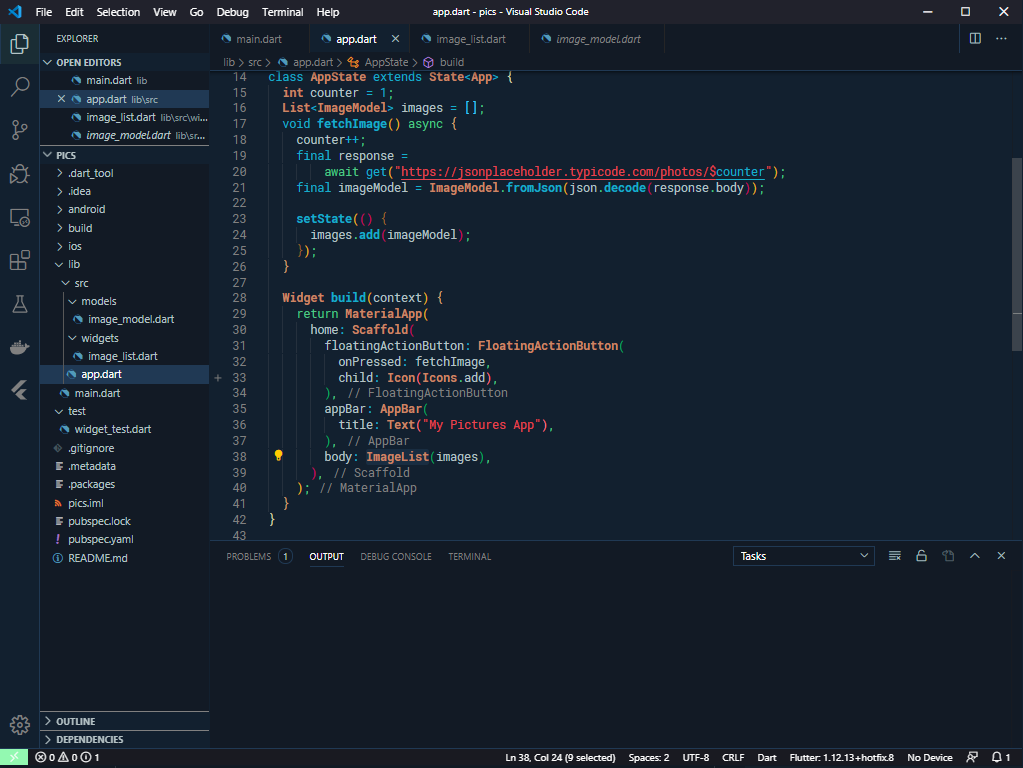
\includegraphics[width=6in]{images/Chapitre3/interface_vs_code.png}
    \label{fig:interfacevscode}
    \caption{Interface du logiciel Visual Studio Code}
\end{figure}
\newpage
\subsection{Developpement}
\subsubsection{Base de données}
Pour la base de données nous avons choisi d'utiliser le service de base de données fourni par
firebase avant d'aller plus dans le détail définissons firebase.

\textbf{Firebase}
Firebase est un ensemble de services d'hébergement pour n'importe quel type 
d'application (Android, iOS, Javascript, Node.js, Java, Unity, PHP, C++ ...).
Il propose d'héberger en NoSQL et en temps réel des bases de données, du contenu,
de l'authentification sociale (Google, Facebook, Twitter et Github), et des 
notifications, ou encore des services, tel que par exemple un serveur de 
communication temps réel.~\cite{Firebase2020}

\begin{figure}[!h]
    \centering
    
\includegraphics[width=8cm]{images/Chapitre3/firebase.png}
    \label{fig:label8}
    \caption{Logo de Firebase}
\end{figure}  
\begin{figure}[!h]

    \centering
    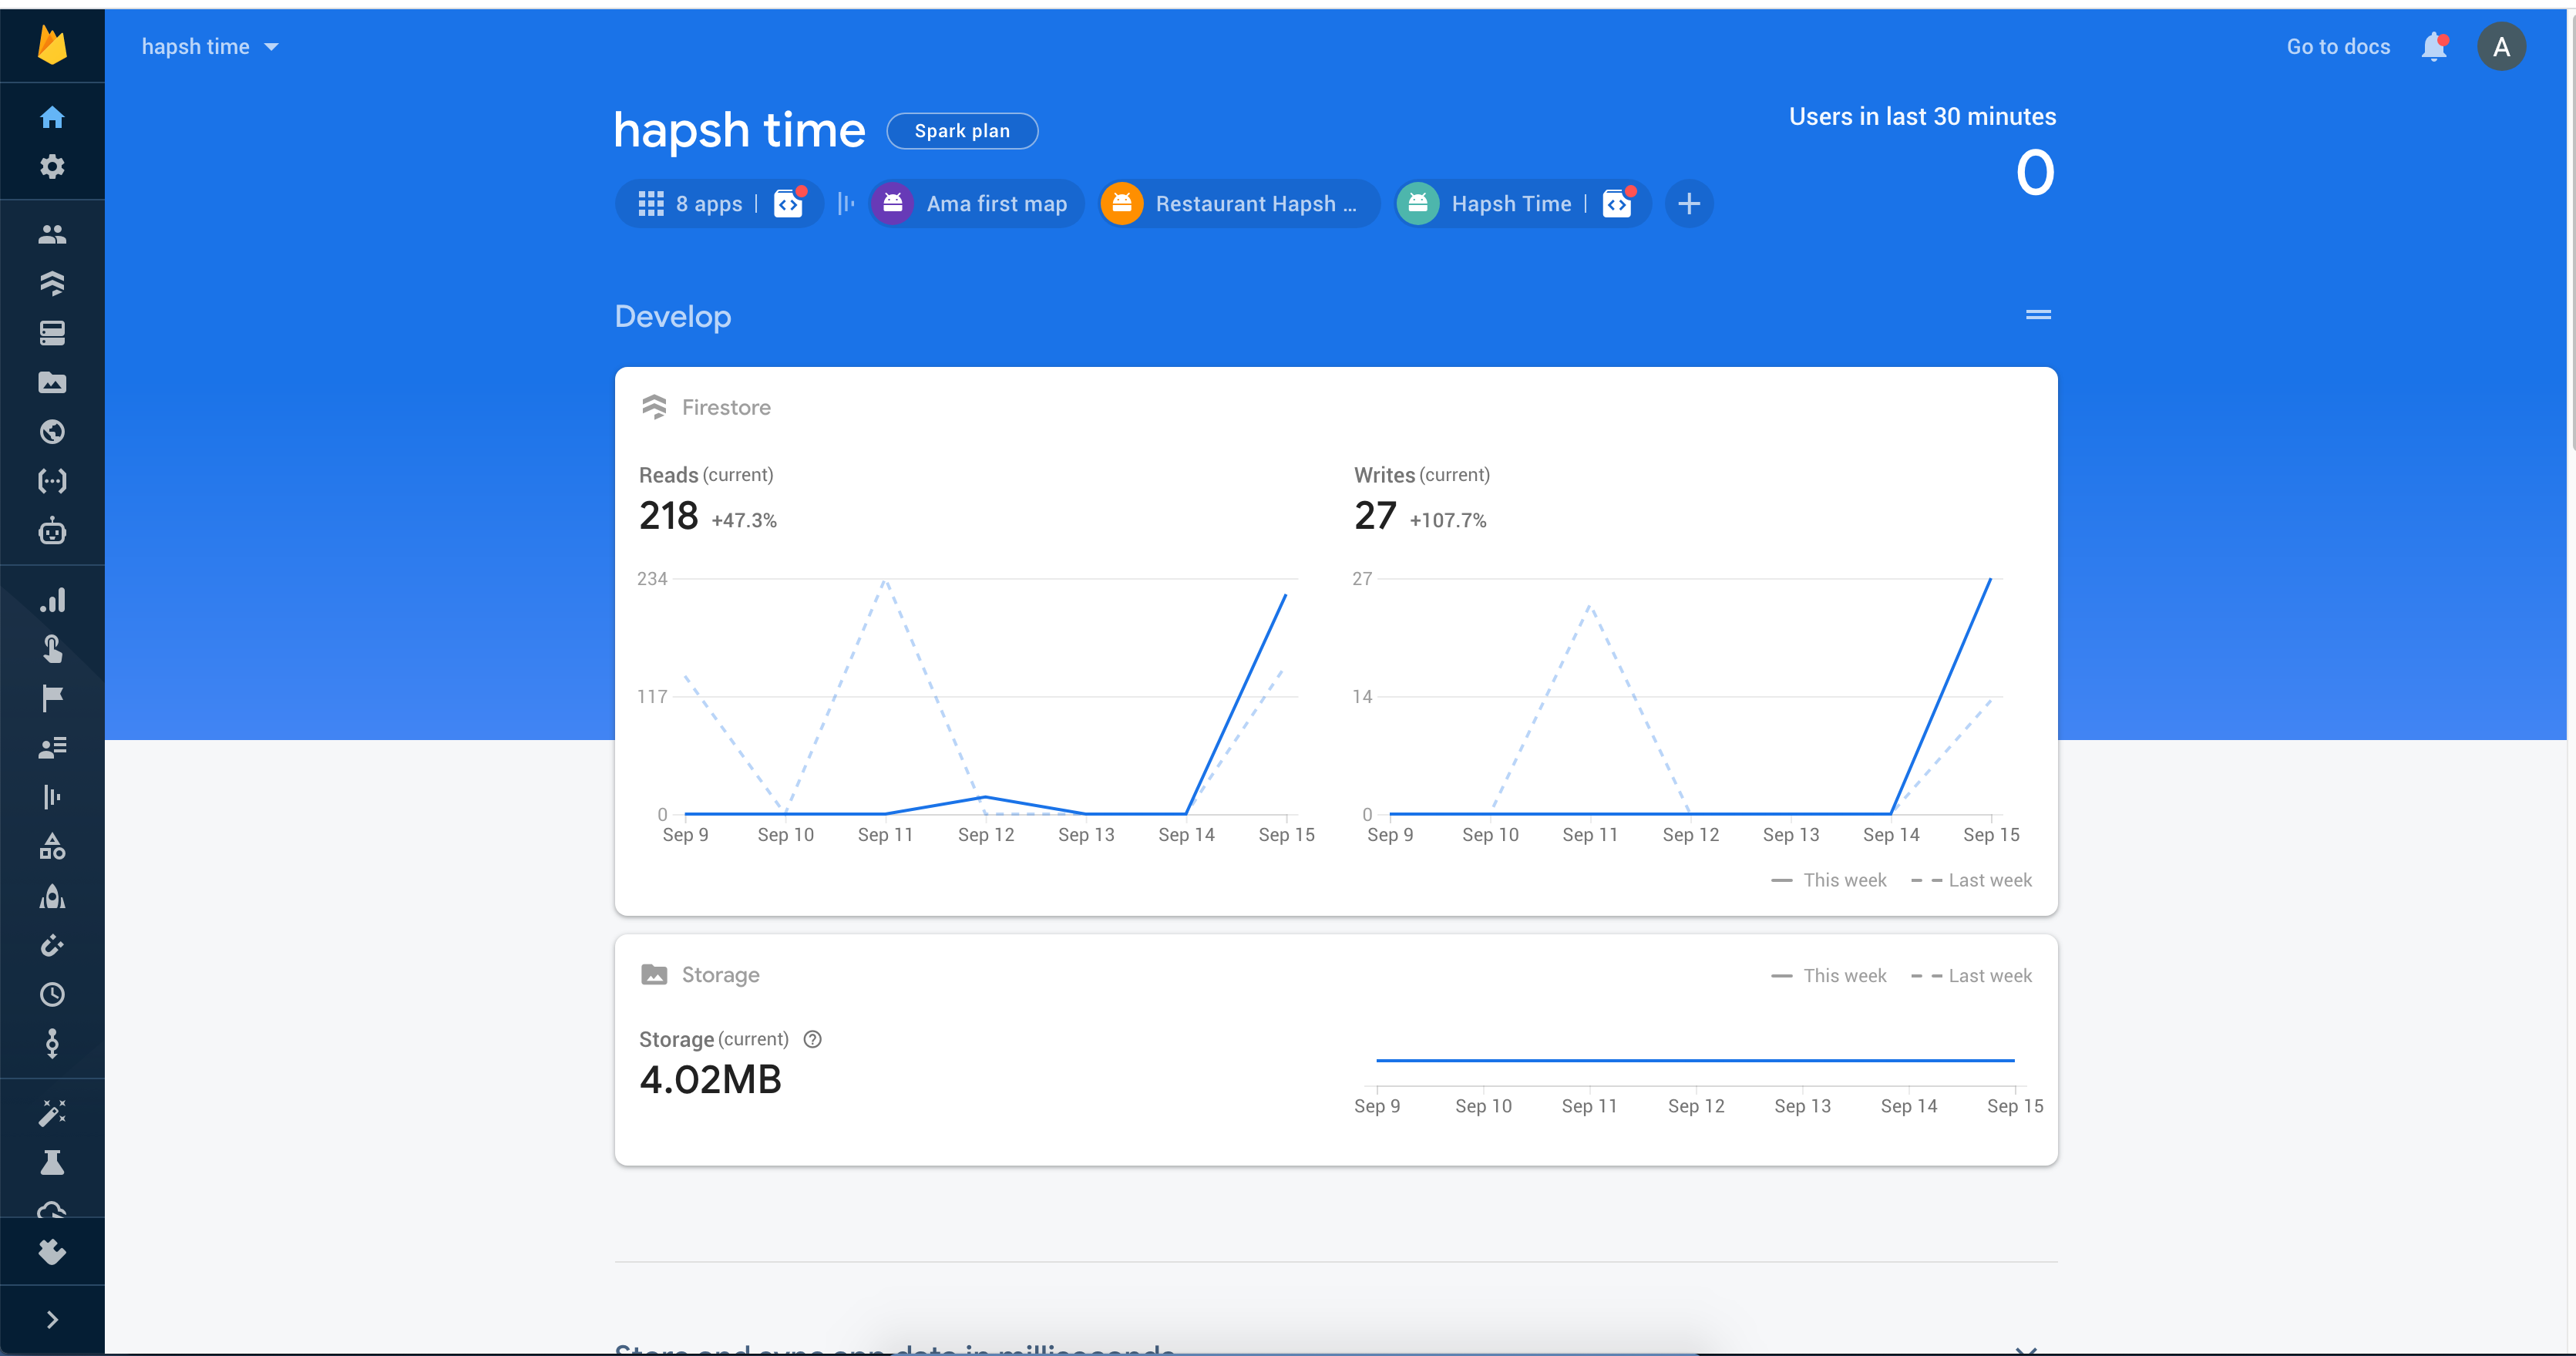
\includegraphics[width=7in]{images/Chapitre3/firebase_console.png}
    \label{fig:firebasepricing}
    \caption{Interface de la console de Firebase }
\end{figure}

\newpage
\subsubsection{Les packages utilisés: }         
\textbf{Google maps flutter:}\\
Avec le plugin Google Maps Flutter, on peut ajouter des cartes basées sur les données de Google Maps ànotre application. Le plugin gère automatiquement l'accès aux serveurs Google Maps, l'affichage de la carte et la réponse aux gestes de l'utilisateur tels que les clics et les traînées. On peut également ajouter des marqueurs à notre carte. Ces objets fournissent des informations supplémentaires sur les emplacements de la carte et permettent à l'utilisateur d'interagir avec la carte.\bigskip

\textbf{Cloud Firestore:}\\
Ce package permet d'intégrer les services de base de données NoSQL de Firebase pour l'utilisation en temps réel. Les données sont stockées dans l'arborescence JSON sous la forme des collections, où chaque collection un nombre infini de documents, ces derniers contiennent les données de la base de données.\bigskip

\textbf{Geolocator: }\\
Geolocator est un plugiciel de géolocalisation dédié à Flutter, ce dernier offre un accès facile au service de localisations spécifiques à la plateforme.\bigskip

Geolocator permet de: 
\begin{itemize}
    \item Obtenir le dernier emplacement de l'utilisateur.
    \item Obtenir l'emplacement actuel de l'appareil.
    \item Vérifier si les services de localisation sont activés sur l'appareil.
    \item Calculer la distance (en mètres) entre deux points géographique.
\end{itemize}
\bigskip

\textbf{Firebase auth:}\\
Firebase auth est un plugin Flutter pour utiliser l'API d'authentification Firebase. Cet APi permet de gérer les authentifications des utilisateurs en offrant differentes options d'inscription et de connexion a leurs comptes.\bigskip

\textbf{Goole sign in:}\\
Google sign in est un plugin Flutter qui offre un système d'authentification sécurisé pour se connecter avec un compte Google sur Android et iOS.\bigskip